\documentclass[a4paper, 12pt]{article}
\usepackage[utf8]{inputenc}
\usepackage{comment}
\usepackage[spanish]{babel}
\usepackage[margin=1.2in]{geometry}
\usepackage{natbib}
\usepackage{graphicx}
\usepackage{placeins}
\usepackage{caption}
\newcommand\tab[1][1cm]{\hspace*{#1}}
\geometry{top = 1in}
\setlength{\textfloatsep}{1\baselineskip plus 0.2\baselineskip minus 0.5\baselineskip}
\setlength{\parindent}{2em}
\renewcommand\textfraction{.1}

\title{Análisis Exploratorio de Datos \\ Trabajo Práctico 1 - Organización de Datos}
\author{Grupo Back to the Data}
\date{22/04/2019}

\begin{document}
\begin{figure}
    \centering
    \makebox[\textwidth]{
\includegraphics[width=250pt]{logofiuba.jpg}}
\end{figure}

\maketitle

\FloatBarrier
\begin{center}
        \begin{tabular}{ |c|c|c| }
          \hline
          Nombre & Padrón & Mail \\
          \hline\hline
          Álvarez, Federico & 99266 & fede.alvarez1997@gmail.com \\
          \hline
          La Torre, Gabriel & 87796 & latorregab@gmail.com \\
          \hline
          Medrano, Lucas Nicolás & 99247 & lucasmedrano97@gmail.com \\
          \hline
          Piro Martino, Ariel & 99469 & ariel.piro@hotmail.com \\
          \hline
        \end{tabular}
\end{center}
\FloatBarrier

\newpage

\tableofcontents
\newpage
\section{Introducción}
	 En el trabajo se hace un análisis exploratorio de un set de datos provistos por la empresa Jampp. En el mismo se encuentra información de subastas, instalaciones, clicks, entre otros.\\
	 Primero se hará una visión general de los archivos installs.csv, clicks.csv, auctions.csv y events.csv para entender la distribución y la cantidad de datos, el significado de las columnas, reconocer las columnas que no aportan información, por ejemplo, las que tienen todos sus valores nulos, y reconocer el tipo de datos en cada columna, seguido de un análisis más profundo para obtener más información de los datos. Luego se hará un análisis global, buscando información relativa a los archivos en conjunto, permitiendo obtener otro tipo de información.

\section{Análisis individual de archivos}
\subsection{Subastas}
	\subsubsection{Análisis general} \label{analisis general}
	  El archivo 'auctions.csv' contiene información acerca de subastas.
	Hay dos columnas que no nos aportan información significante. 'auction\_type\_id' tiene todos sus valores 		nulos, por lo que no fue tomada en cuenta para el análisis. 'country' informa un solo valor posible.

	 La columna platforms tiene dos valores posibles (1 y 2) que se supone son Android e iOS. Va a ser importante para el análisis que hagamos más adelante. De ahora en más, platform y sistema operativo serán sinónimos en este informe.

	 Por último, 'source' nos da información acerca del exchange de donde surge la subasta.

	 Además vemos que ningún valor de este archivo, excluyendo la columna 'auction\_type\_id', es nulo, por lo que no es necesario tomar ninguna decisión respecto a eso.

	\subsubsection{Análisis de los dispositivos en las subastas}
	 Un punto muy importante para analizar son los dispositivos. Esto trajo un problema al analizar los datos y puede cambiar la forma en la que se entienden los mismos.
	Podemos, por ejemplo, ver el top diez de dispositivos de los cuales se generan más subastas.
	\FloatBarrier
		\begin{figure}
			\centering
			\makebox[\textwidth]{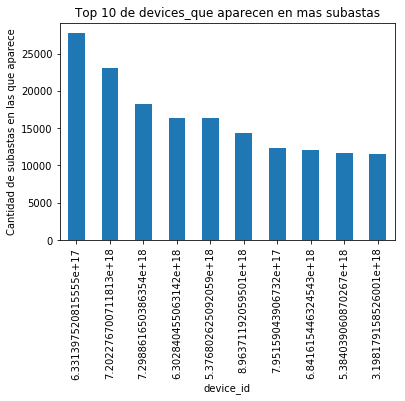
\includegraphics[width=350pt]{images/auctions/top10devicessubastas.png}}
		   	\caption{Top 10 de dispositivos con mayor cantidad de subastas}
			\label{top10devicessubastas}
		\end{figure}
	\FloatBarrier

	 Ahora el problema.\newline
	 En total, en las 19571319 subastas, aparecen 206171 dispositivos. Algo interesante sería conocer cuántos tienen cada plataforma. Por lo que hacemos un gráfico.

	\FloatBarrier
		\begin{figure}
			\centering
			\makebox[\textwidth]{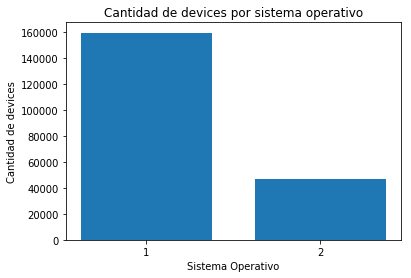
\includegraphics[width=350pt]{images/auctions/devicesporSO.png}}
		   	\caption{Cantidad de dispositivos para cada plataforma}
			\label{devicesporSO}
		\end{figure}
	\FloatBarrier

	 Al obtener los datos del gráfico, observamos que la suma de las cantidades de dispositivos para cada plataforma es 206453. ¡Esto es mayor a la cantidad total de dispositivos (206171)!\newline
	 La causa de este problema se entiende al conocer cómo se obtuvieron las cantidades. Primero se contó la cantidad de dispositivos total. Luego se separaron los que tuvieran plataforma '1' de los que tuvieran plataforma '2' (tener en cuenta que como hay una fila por subasta, cada dispositivo puede aparecer en filas distintas). Al sumar ambas cantidades obtenemos un número mayor que el total, por lo que es evidente que hay dispositivos que tienen ambas plataformas, es decir, en algúnas filas aparecen con un valor de la columna 'platform' y en otras filas con otro.

	 Haciendo una simple resta, se puede ver que la cantidad de dispositivos que aparecen con plataformas distintas es 282, y que en total participan en 47862 subastas. De hecho hay un dispositivo (5.292967062497395e+18) que aparece en el top 300 de cantidad de subastas.

	 Esto puede alterar los análisis que incluyen división en plataformas. Sin embargo, no es trivial que haya que borrar estos datos, porque se estarían borrando casi 50000 subastas. Además, dejar los datos como están no altera a los estudios que se hagan sin dividir el problea por sistemas operativos. Por lo tanto se decidió trabajar de la siguiente manera.
	\begin{itemize}
		\item En aquellos análisis que, a priori, no parezcan ser afectados por estos errores en las plataformas de los dispositivos usaran el dataset entero.
		\item En los restantes, se usará un dataframe filtrado, en el que no están los dispositivos conflictivos.
	\end{itemize}
	
	 Igualmente, se compararon los gráficos conflictivos para el dataframe original y el filtrado, y no había diferencias substanciales cualitativas ni cuantitativas.
	
	
	\subsubsection{Subastas por día de Marzo}
	 Como primer acercamiento a este set de datos, es interesante ver cómo se distribuye la cantidad de subastas en los días que incluye el archivo (05/03/19 al 13/03/19). El gráfico \ref{subastasmarzo} representa dicha distribución. En él se pueden observar varias cosas:
	\begin{itemize}
		\item La cantidad de subastas parece, en general, aumentar con el paso de los dias.
		\item El valor del último día es más del doble del valor del primer día.
		\item El mayor aumento se da del sexto al septimo día.
		\item La cantidad de subastas varía entre unos valores extremos, aproximados, de un millón y 3 millónes.
	\end{itemize}

	\FloatBarrier
		\begin{figure}
			\centering
			   	\makebox[\textwidth]{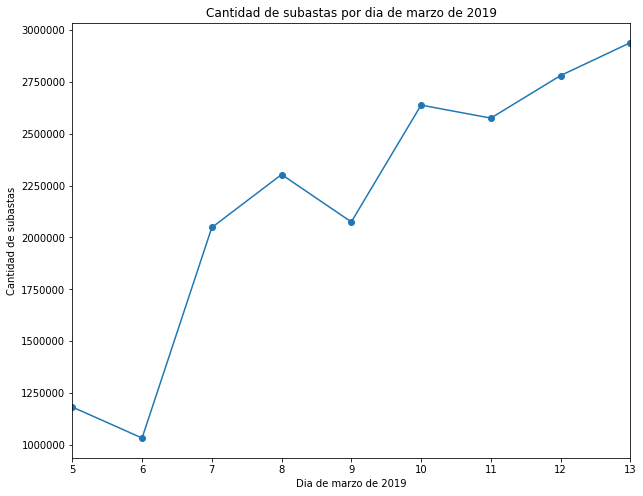
\includegraphics[width=300pt]{images/auctions/subastaspordia.png}}
		   		\caption{Cantidad de subastas por día de Marzo}
			   	\label{subastasmarzo}
		\end{figure}
	\FloatBarrier

	\subsubsection{Subastas por día de Marzo por sistema operativo}
	 Otro punto interesante es dividir el problema. Obtener la distribución de subastas en los días con datos disponibles para cada plataforma (Android e iOS). En la imagen \ref{subastasmarzoSO} se pueden observar las cantidades. Observese que llamamos '1' y '2' a las plataformas, ya que no sabemos cuál es Android y cuál es iOS.

	 Puntos interesantes a reconocer:

	\begin{itemize}
		\item Para este análisis se usaron los datos filtrados, ya que los devices que tienen ambas plataformas pueden generar ruido.
		\item La cantidad de subastas para la plataforma '1' es, salvo en el cuarto y el quinto día, considerablemente mayor a la cantidad para la plataforma '2'.
		\item La figura de la plataforma '2' es mucho más ``chata'' que la de la plataforma '1', la cual representa más picos y saltos.
		\item La figura de la plataforma '1' es muy parecida a la del gráfico \ref{subastasmarzo}, mientras que la de la plataforma '2' no lo es. Esto es resultado, principalmente, de lo indicado en el primer ítem. Este análisis puede llegar a ser muy útil para reconocer partes de los datos que son representativas del total.
	\end{itemize}

	\FloatBarrier
	\begin{figure}
			\centering
	   		\makebox[\textwidth]{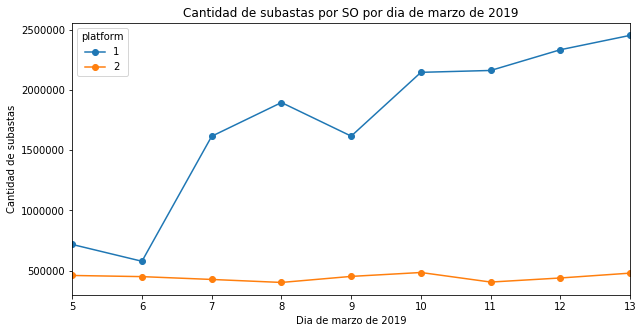
\includegraphics[width=350pt]{images/auctions/subastaspordiaporSO_corregido.png}}
		   	\caption{Cantidad de subastas por día de Marzo y por sistema operativo}
		   	\label{subastasmarzoSO}
		\end{figure}
	\FloatBarrier

	\subsubsection{Subastas por hora del día}
	 Ahora vamos a analizar cómo se distribuyen las subastas a lo largo del día. Para esto hacemos un gráfico de hora del día contra cantidad de subastas (Gráfico \ref{subastashora}).\newline
	 Desde un análisis cualitativo se pueden observar algúnos puntos:
	\begin{itemize}
		\item Parece ser que la mayor cantidad de subastas se distribuyen por la noche y la madrugada.
		\item La cantidad de subastas es poca en horas de la mañana y el mediodía. En el gráfico se puede ver un gran valle en esa parte del día.
	\end{itemize}

	\FloatBarrier
		\begin{figure}
			\centering
			\makebox[\textwidth]{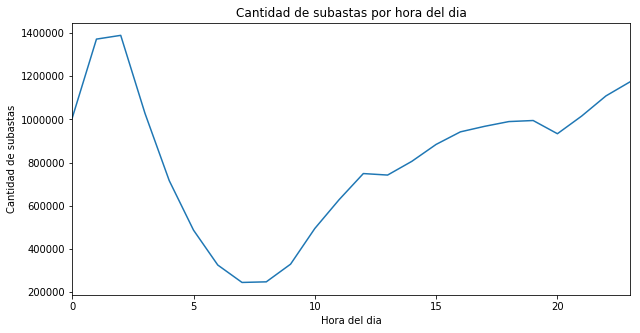
\includegraphics[width=350pt, bb=0 0 640 480]{images/auctions/subastasporhora.png}}
		   	\caption{Cantidad de subastas por hora del día}
			\label{subastashora}
		\end{figure}
	\FloatBarrier
	\subsubsection{Subastas por hora del día por sistema operativo}
	 Al igual que se hizo antes podemos dividir el gráfico para ambas plataformas. Vemos que pasa algo muy parecido que lo que pasaba para la cantidad de subastas por día. El gráfico de la plataforma '1', al tener una cantidad mucho mayor de subastas, es la que predomina en el gráfico de la sección "Subastas por hora del día", y por eso sus gráficos son tan parecidos. El gráfico de la plataforma '2' es bastante más chato, y con cantidades de subastas mucho más chicas.
	En esta subsección y en la siguiente usaremos los datos filtrados.
	\FloatBarrier
		\begin{figure}
			\centering
			\makebox[\textwidth]{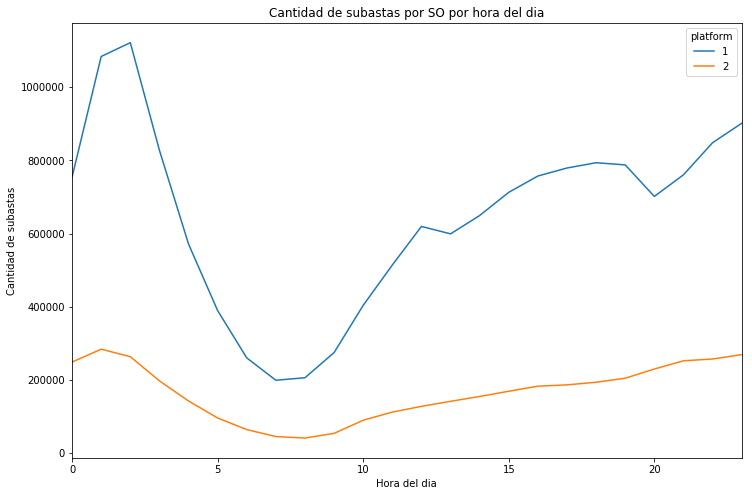
\includegraphics[width=350pt]{images/auctions/subastasporhoraSO_corregido.png}}
		   	\caption{Cantidad de subastas por hora del día por sistema operativo}
			\label{subastashoraSO}
		\end{figure}
	\FloatBarrier

	\subsubsection{Subastas por sistema operativo}
	 Resulta interesante conocer cuál es el sistema operativo para el cual se generan más subastas. Es algo que ya se venía viendo en la forma y nivel (cantidad de subastas) de los gráficos anteriores. Sin embargo, los gráficos vistos hasta ahora no dan un conocimiento directo de la relación de las cantidades de subastas de ambas plataformas.

	 En las figuras que se ven a continuación podemos confirmar que lo que indicabamos en los gráficos anteriores era cierto. La cantidad de subastas es mucho mayor para la plataforma '1'. Además, ahora tenemos una visión más cuantitativa de esta relación, en la imagen \ref{subastasSOporcentajes} vemos una relación porcentual, mientras que la imagen \ref{subastasSOcantidades} nos da más idea de las cantidades.

	\FloatBarrier
		\begin{figure}
			\centering
			\makebox[\textwidth]{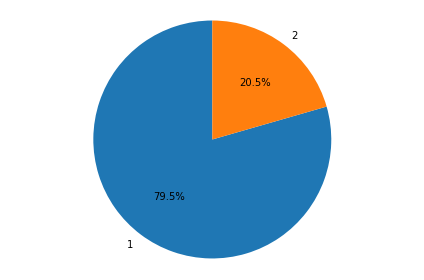
\includegraphics[width=350pt]{images/auctions/subastasporSO_corregido.png}}
		   	\caption{Porcentaje de subastas para cada plataforma}
			\label{subastasSOporcentajes}
		\end{figure}
	\FloatBarrier

	\FloatBarrier
		\begin{figure}
			\centering
			\makebox[\textwidth]{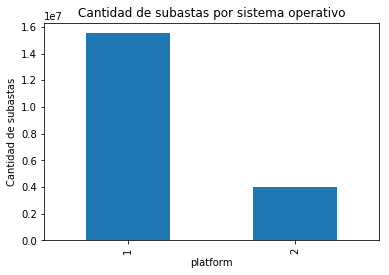
\includegraphics[width=350pt]{images/auctions/subastasporSOcantidad_corregido.png}}
		   	\caption{Porcentaje de subastas para cada plataforma}
			\label{subastasSOcantidades}
		\end{figure}
	\FloatBarrier

	\subsubsection{Subastas por source}
	 Como indica la introducción a esta sección (vease \ref{analisis general}), source nos indica el exchange que generó la subasta. Se puede obtener, a partir de los datos, cuáles son los exchanges principales, y cuántas subastas generan.

	 A tener en cuenta:
	\begin{itemize}
		\item Los que se muestran son todos los exchanges que aparecen en el archivo.
		\item Al igual que en las plataformas, los exchanges se toman por un id, y no por su nombre.
		\item Hay una clara diferencia en las cantidades.
		\begin{itemize}
			\item El exchange '0' es predominante, superando ampliamente el millón de subastas generadas.
			\item El siguiente, source '1', aunque es mucho menor que el '0', sigue superando a los demas exchange por una gran cantidad. Llegando a las 400000 subastas generadas
			\item Los exchanges '2', '5' y '6' parecen no tener mucho peso en el gráfico. Aunque quizás podría tomarse la cantidad del '5' como significativa.
		\end{itemize}
	\end{itemize}

	\FloatBarrier
		\begin{figure}
			\centering
			\makebox[\textwidth]{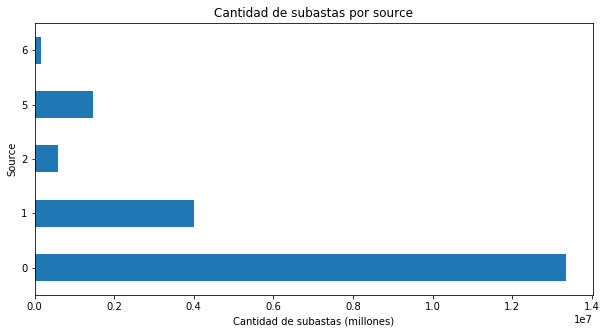
\includegraphics[width=\textwidth]{images/auctions/subastasporsource.png}}
		   	\caption{Cantidad de subastas para cada source}
			\label{subastassource}
		\end{figure}
	\FloatBarrier

\clearpage
\subsection{Clicks}
	\subsubsection{Análisis General}
		
		 En el archivo \texttt{clicks.csv} se nos muestran los clicks que se realizaron entre el 5 y el 13 de Marzo de este año. Este csv cuenta con 20 columnas y 26000 filas aproximadamente. En las columnas tenemos datos como en qué latitud y longitud se hizo el click, cuánto tardó el usuario en hacer el click, de qué país es el dispositivo, en qué parte de la pantalla del celular se realizó click, entre otras cosas.
		
		 En primera medida sacamos las columnas que no nos aportaban nada. La columna action\_id tenía todos NaN así que fue removida. La columna que indicaba el país solo daba como resultado un país unicamente así que nos pareció irrelevante y la quitamos. Así también eliminamos la columna de wifi\_connection ya que todas daban False, lo cual es un poco raro, porque esto indicaría ninguno estaba conectado a wifi. Finalmente se sacó la columna trans\_id ya que era un identificador único para cada uno de los clicks y para analizar este archivo solo no nos aportaba nada.
		
		 También, se tomó la decisión de cambiar los tipos de algúnas columnas para ahorrar más espacio. Las columnas advertiser\_id y source\_id se las cambió a category ya que tenían pocos valores y siempre eran los mismos. Y a varias de las columnas se las pasó de float64 a float32, ya que no necseitaban tantos bits para representar sus datos.
	\subsubsection{Clicks en los distintas publicidades}
		 Se van a observar la cantidad de clicks en las distintas publicidades

		\FloatBarrier
		\begin{figure}[h]
			\centering
			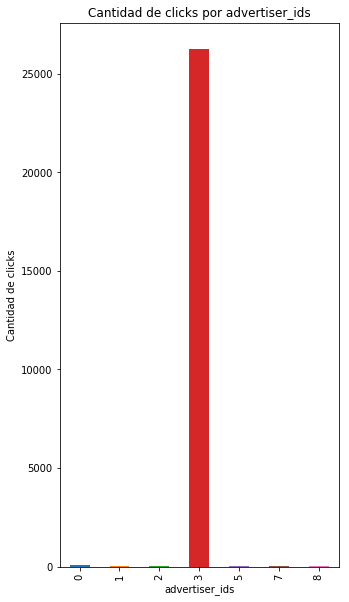
\includegraphics[scale=0.5]{images/clicks/clicks_advertiser_id.png}
			\caption{Clicks en los advertiser\_id}
		\end{figure}
		\FloatBarrier

		 Se puede observar que prácticamente todos son clicks en la publicidad con el id 3. El porcentaje de clicks en este id es de 99.7. Al parecer, le sirve mucho más a Jampp mostrar las publicidades del id 3 o es una publicidad de una app que es más común que todos usen.

	\subsubsection{Clicks en los source\_id}
		 En este gráfico vamos a mostrar la cantidad de clicks que se hacen en los distintos source\_id que hay en el archivo
		
		
		\FloatBarrier
		\begin{figure}[h]
			\centering
			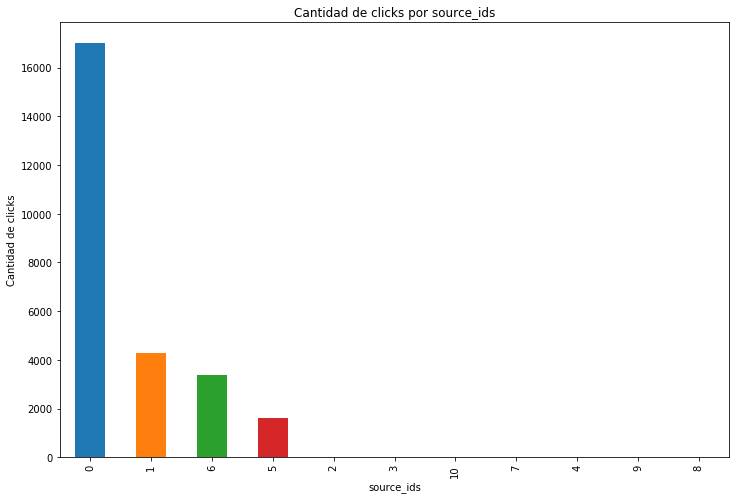
\includegraphics[width=\textwidth]{images/clicks/clicks_source_id.png}
			\caption{Clicks en los source\_id}
		\end{figure}
		\FloatBarrier

		 Como se puede observar la mayoría de los clicks estan distribuidos entre los id 0, 1, 6 y 5 siendo el source\_id 1 el que más cantidad de clicks tiene.


	\subsubsection{Clicks en los carrier\_id}
		 En el siguiente gráfico se mostrará la cantidad de clicks que tiene cada carrier\_id
		
		\FloatBarrier
		\begin{figure}[h]
			\centering
			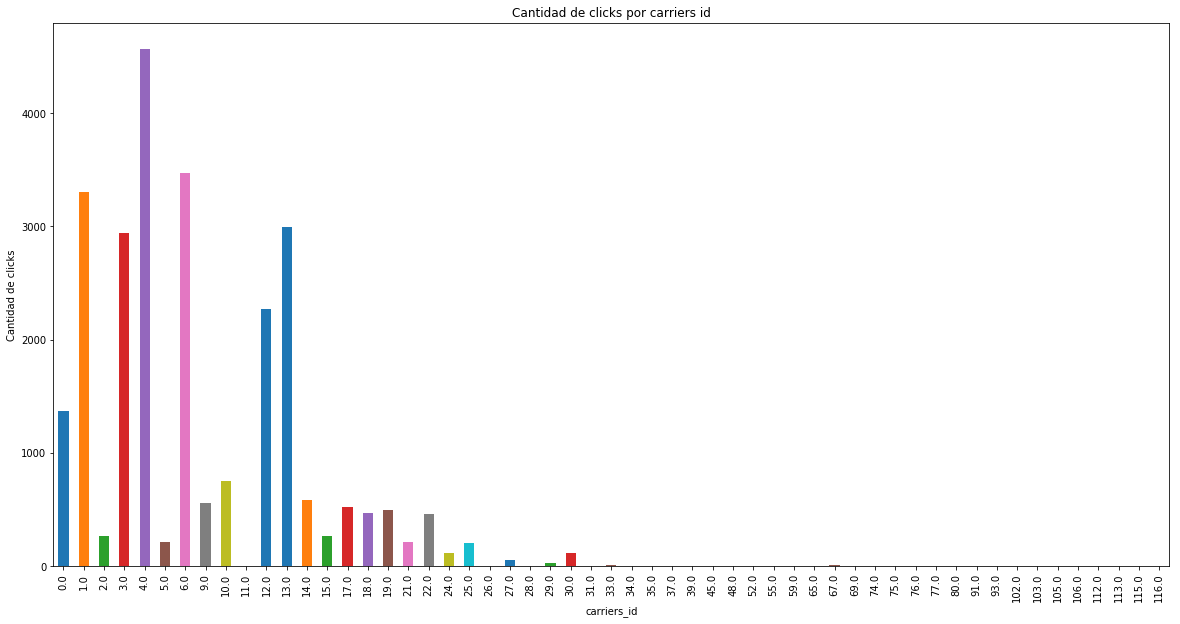
\includegraphics[width=\textwidth]{images/clicks/clicks_carrier_id.png}
			\caption{Clicks en los carrier\_id}
		\end{figure}
		\FloatBarrier

		 Por más que hay varios carrier\_id se ve que la mayoría de clicks se distribuyen en aproximadamente 20 carriers\_id. El carrier\_id que más realiza clicks es el 4.0.

	\subsubsection{Clicks en los os\_minor}
		 Se mostrará en este gráfico la cantidad de clicks que realizan los dispositivos que tienen ciertas mínimas versiones de sus sistemas operativos.

		\FloatBarrier
		\begin{figure}[h]
			\centering
			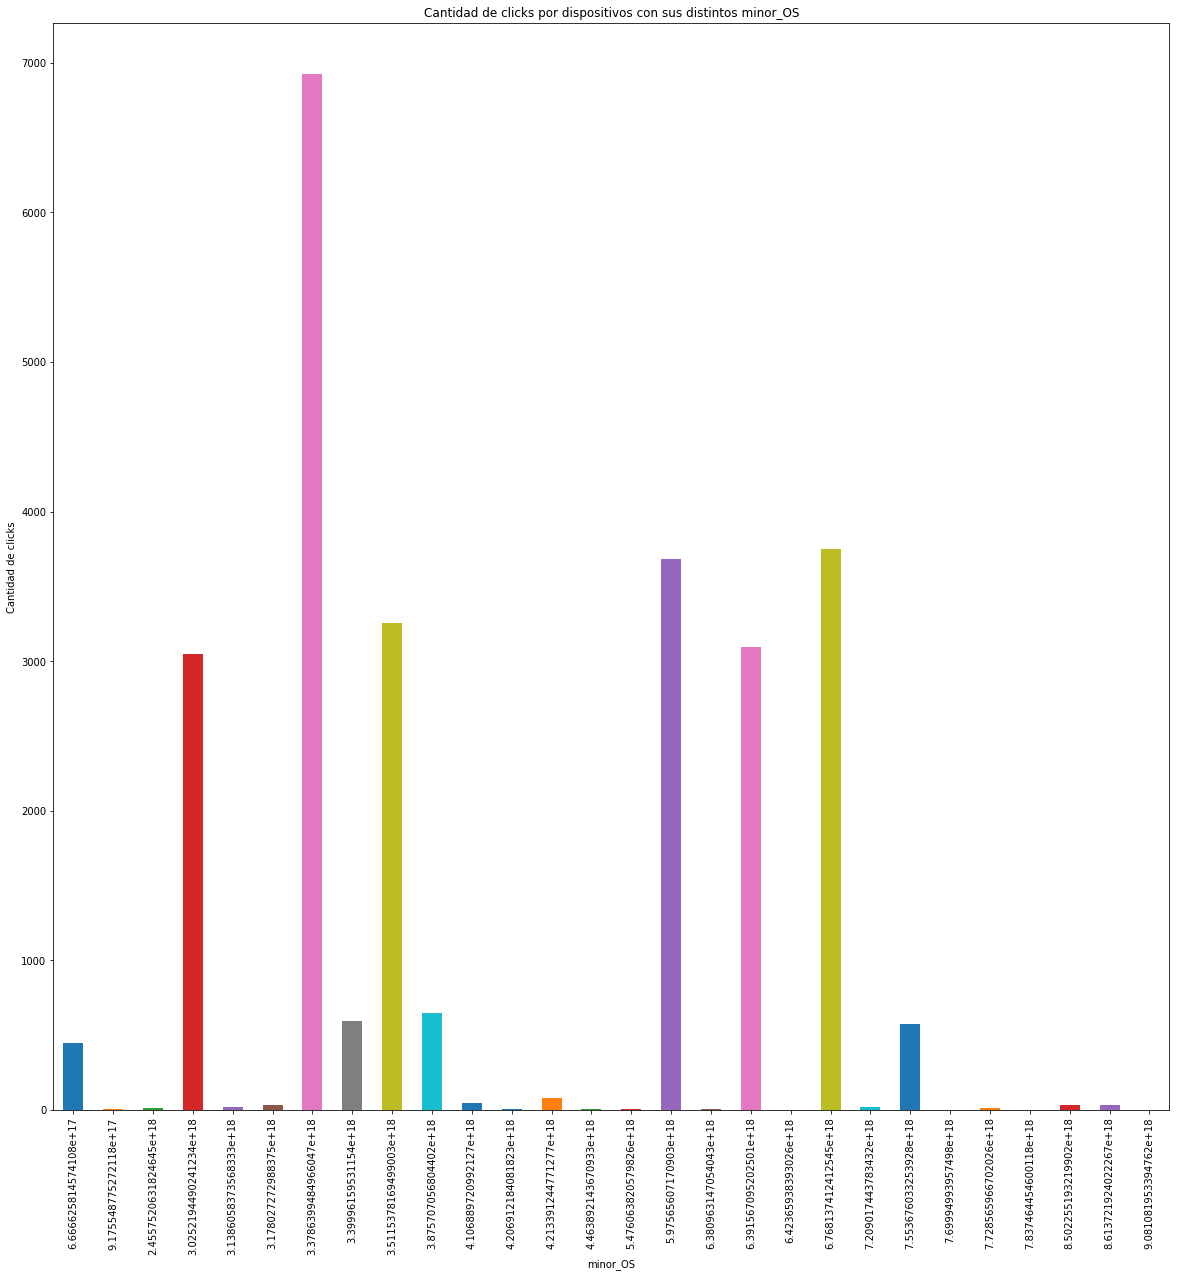
\includegraphics[scale = 0.37]{images/clicks/clicks_minor_OS.png}
			\caption{Clicks en los os\_minor}
		\end{figure}
		\FloatBarrier

		 Vemos que la cantidad de clicks es liderada por los dispositivos con un os\_minor 3.378640e+18.

	\subsubsection{Clicks en los os\_major}
		 Se mostrará en este gráfico la cantidad de clicks que realizan los dispositivos que tienen ciertas máximas
		versiones de sus sistemas operativos.

		\FloatBarrier
		\begin{figure}[h]
			\centering
			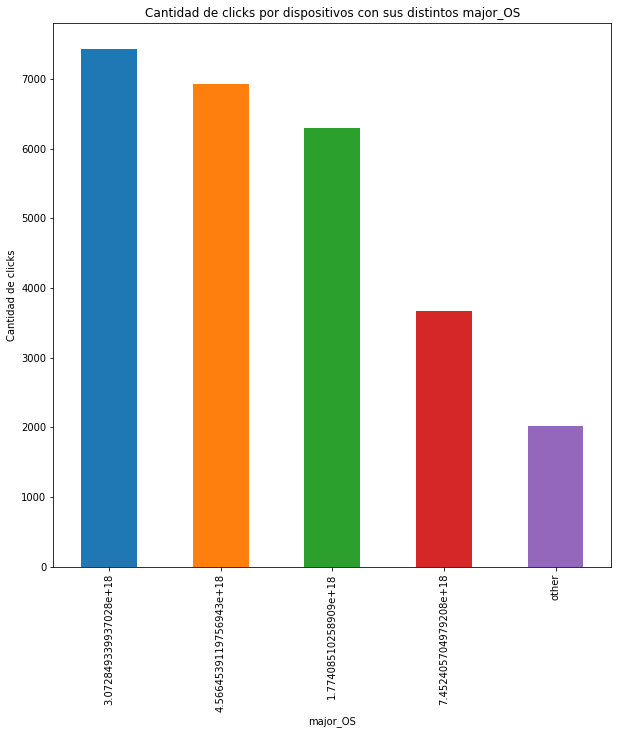
\includegraphics[scale = 0.5]{images/clicks/clicks_major_OS.png}
			\caption{Clicks en los os\_major}
		\end{figure}
		\FloatBarrier

		 En este casos se reparte bastante equitativamente la cantidad de clicks en cuatro distintos os\_major.
		No podemos saber cuanto es la cantidad total de los os\_major debido a que una categoría es ``others'' y no sabemos
		cuántos distintos sistemas operativos tiene encerrado ese término.

	\subsubsection{Clicks en los agent\_device}
		 En este caso notamos que la cantidad de agent\_device es mucha. Hay un total de 190 diferentes agent\_device
		y la mayoría de sus datos son NaN. Solamente posee alrededor de 3000 datos. Por lo tanto, llegamos a la conclusión
		de que no aporta ningún dato importante ni tampoco es confiable la información que dé ya que la cantidad de datos
		que tiene es muy poca.

	\subsubsection{Clicks en los spec\_brands}
		 A continuación mostraremos un gráfico donde podemos ver la cantidad de clicks que tienen los distintos spec\_brands.

		\FloatBarrier
		\begin{figure}[h]
			\centering
			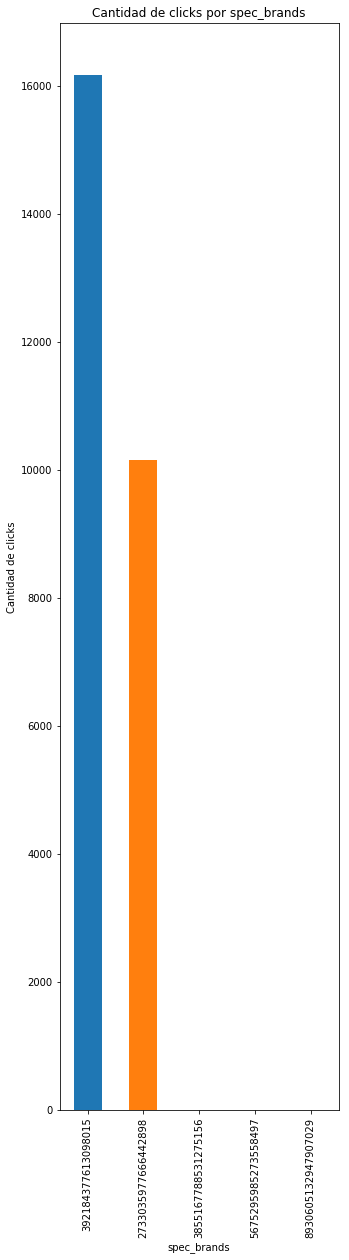
\includegraphics[scale = 0.7]{images/clicks/clicks_specs_brand.png}
			\caption{Clicks en los spec\_brands}
		\end{figure}
		\FloatBarrier

		 Por más que hay 5 spec\_brands, se ve claramente que los clicks se realiazan practimacmente dos spec\_brands.
		Estos son 392184377613098015 y 2733035977666442898.
		

	\subsubsection{Clicks en las distintas marcas}
		 Este gráfico nos muestra la cantidad de clicks en las distintas marcas de celular.

		\FloatBarrier
		\begin{figure}[h]
			\centering
			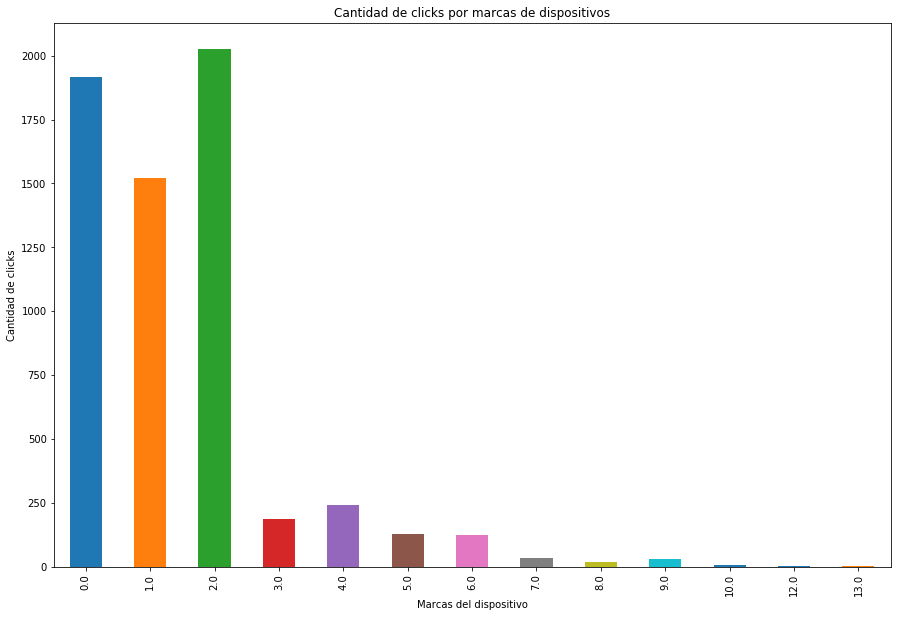
\includegraphics[width=\textwidth]{images/clicks/clicks_brand.png}
			\caption{Clicks en las distintas marcas de teléfono}
		\end{figure}
		\FloatBarrier

		 Como se puede observar, hay un total de 13 marcas distintas de teléfonos y la mayoría de clicks la realizan
		celulares de la marca 2.0, 0.0 y 1.0.

	\subsubsection{Clicks en Android e IOS}
		 En el siguiente gráfico se muestra la cantidad de clicks que tienen los celulares con Android o IOS.

		\FloatBarrier
		\begin{figure}[h]
			\centering
			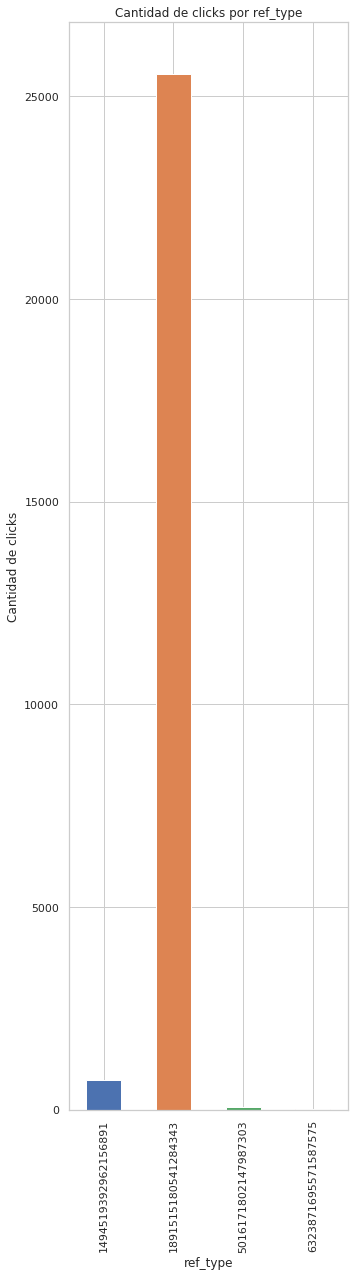
\includegraphics[scale = 0.6]{images/clicks/clicks_ref_type.png}
			\caption{Clicks en las distintos sistemas operativos}
		\end{figure}
		\FloatBarrier

		 Algo raro que se observa es que hay un total de cuatro sistemas operativos. Esto esta mal debido aque solo
		debería haber Android o IOS. Por lo tanto, se puede concluir que los dos valores que menos clicks tienen son datos
		erróneos. Es decir, solo hay que tener en cuanta los que clicks que tienen como sistema operativo los dos que más
		clicks concentran en este gráfico.

	\subsubsection{Clicks en ref\_hash}
		 El ref\_hash nos muestra un id único de cada dispositivo que realiza click. Encontramos que hay ciertos ref\_hash que se
		repiten varias veces. Por ejemplo, el que más veces lo hace, realiza un total de 41 clicks. La verdad es que es
		muy raro que una persona toque click 41 veces en 9 días. Por lo tanto, no podemos descartar que esos casos con
		muchos clicks sea un fraude. Hay muchísimos que tienen más de 10 clicks. Es información que hay que manejar con
		cuidado ya que uno no sabe si son usuarios de verdad. Son números difíciles de creer a priori, basándonos en la
		experiencia personal y la intuición, pero, aunque improbables, no son imposibles.


	\subsubsection{Clicks en los dias y horas}
		En este primer gráfico se puede ver la evolución de la cantidad de clicks que se hicieron entre los dias 5 y 13 de Marzo

		\FloatBarrier
		\begin{figure}[h]
			\centering
			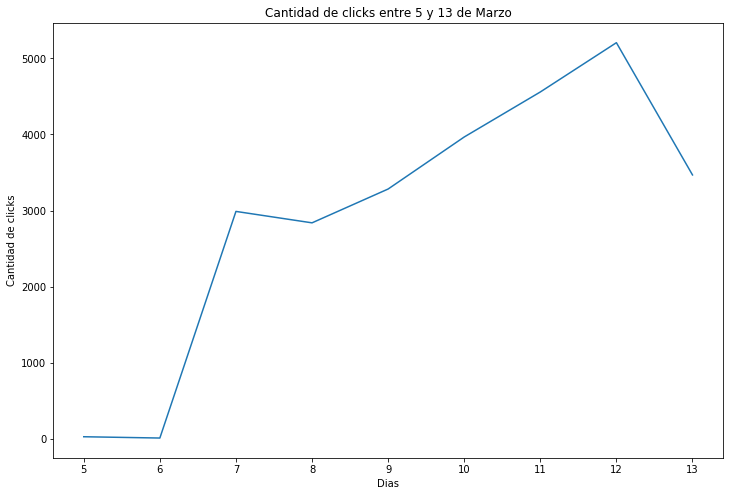
\includegraphics[width=\textwidth]{images/clicks/clicks_days.png}
			\caption{Clicks entre 5 y 13 de Marzo}
		\end{figure}
		\FloatBarrier

		 Se observa que la cantidad de clicks empieza a aumentar a partir del día 8 y sube hasta alcanzar su máximo el día 12 y luego baja.
		\clearpage
		 Ahora vamos a mostrar un gráfico que indica la cantidad de clicks distribuidos en las distintas horas del día.

		\FloatBarrier
		\begin{figure}[h]
			\centering
			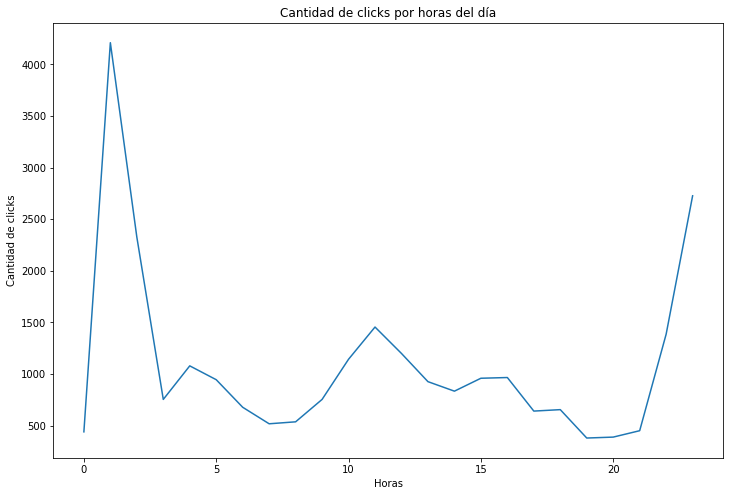
\includegraphics[width=\textwidth]{images/clicks/clicks_hours.png}
			\caption{Clicks en las horas del día}
		\end{figure}
		\FloatBarrier
		
		 En este gráfico se ve claramente que la cantidad de clicks suben exageradamente cuando llega la noche, más precisamente entre las 8pm y las 2am. Se podría decir que la gente utiliza más el celular a estas horas.
		\newline
		\newline
		 En este gráfico de áreas se muestan la cantidad de clicks por hora en el día de los distintos advertiser\_id
	
		\FloatBarrier
		\begin{figure}[h]
			\centering
			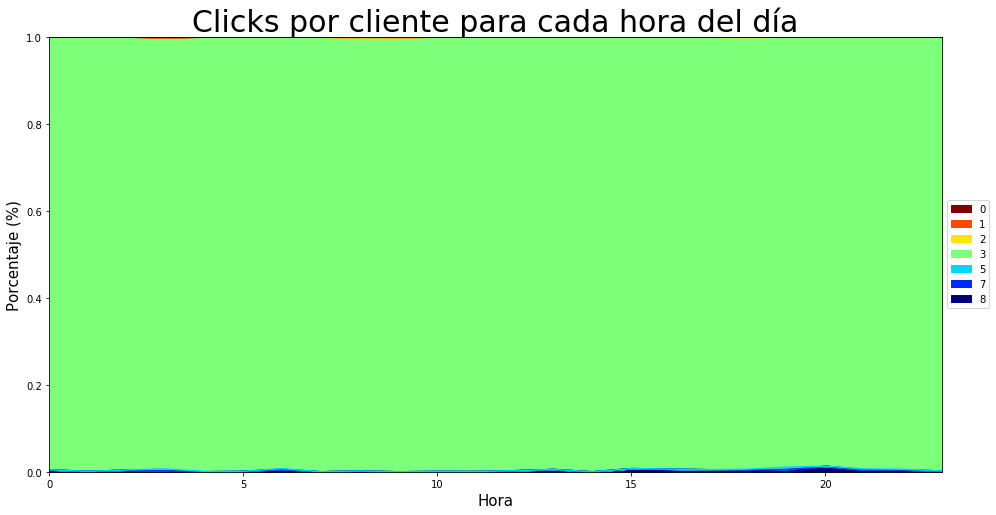
\includegraphics[scale=0.37]{images/clicks/clicks_advertiser_id_hours_persentage.png}
			\caption{Clicks en las horas del día de los advertiser\_id (Porcentaje)}
		\end{figure}
		\FloatBarrier



		 Se puede ver, como se esperaba, que prácticamente toda el área esta pintada del advertiser id 3 que es el que más abunda en este archivo.
		\newline
		\newline
		 El siguiente gráfico muestra la cantidad de clicks en las distintas horas del día de los source\_id que se encuentran en este archivo.

		\FloatBarrier
		\begin{figure}[h]
			\centering
			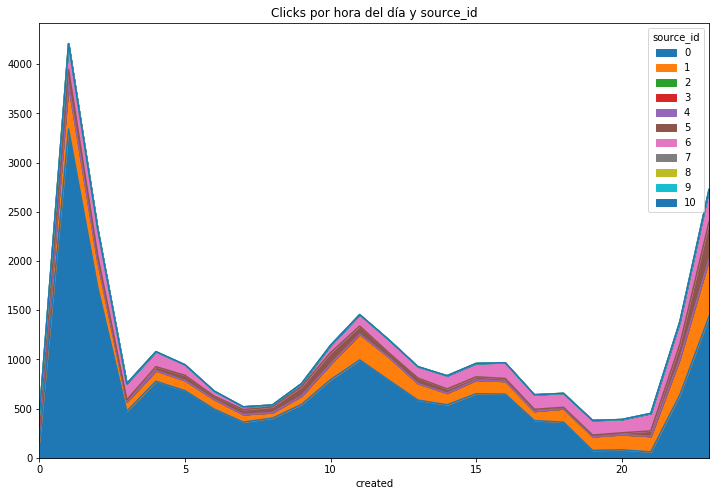
\includegraphics[width=\textwidth]{images/clicks/clicks_source_id_hours.png}
			\caption{Clicks en las horas del día de los source\_id}
		\end{figure}
		\FloatBarrier

	
		 No se ve diferencia en cómo evoluciona la cantidad de clicks de los distintos source\_id dependiendo la hora del día. No obstante, se puede observar que la mayoría de los clicks son de los source\_id 0, 1, 5, 6.

		\clearpage
		 Este nuevo gráfico nos mostrará los clicks en las horas del día distribuidos en los distintos specs\_brand existentes.

		\FloatBarrier
		\begin{figure}[h]
			\centering
			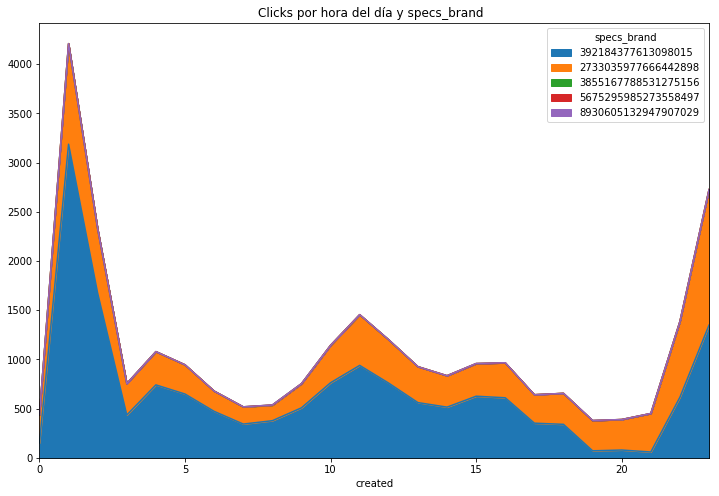
\includegraphics[width=\textwidth]{images/clicks/clicks_specs_brand_hours.png}
			\caption{Clicks en las horas del día de los specs\_brand}
		\end{figure}
		\FloatBarrier

		 La cantidad de clicks se concentra en los specs\_brand 392184377613098015 y 2733035977666442898 que son los que predominan en el csv.
	
	\clearpage
	\subsubsection{Posición geográfica del click}
		
		 En estos gráficos mostraremos las latitudes y longitudes de los clicks efectuados.

		\FloatBarrier
		\begin{figure}[h]
			\centering
			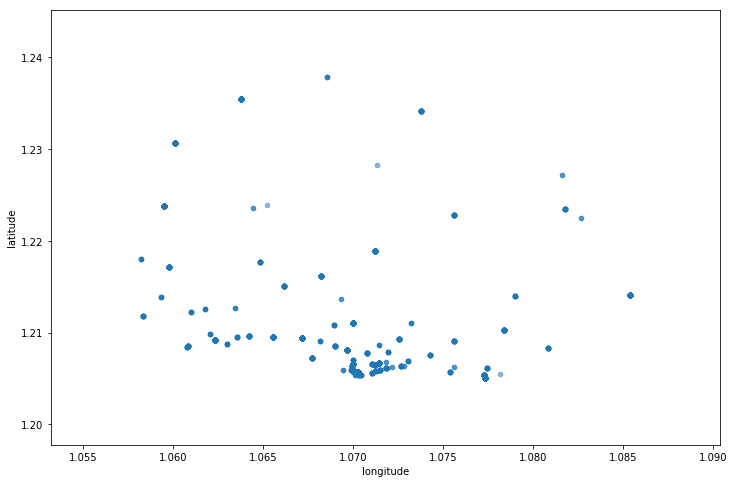
\includegraphics[scale=0.48]{images/clicks/clicks_lat_long_scatter.png}
			\caption{Latitud y longitud del click}
		\end{figure}
		\FloatBarrier


		 Se ve que se concentran muchos clicks entre las latitudes 1.21 y 1.20 que intersecan con la longitud 1.07 y alrededores. Posiblemente sea una ciudad más poblada.
		\newline
		\newline
		\newline
		\newline
		\newline
		 En este gráfico se vuelve a mostrar la latitud y la longitud de los clicks pero en este caso identificaremos los clicks con la mayor version de sistema operativo que tiene el dispositivo
		
		\FloatBarrier
		\begin{figure}[h]
			\centering
			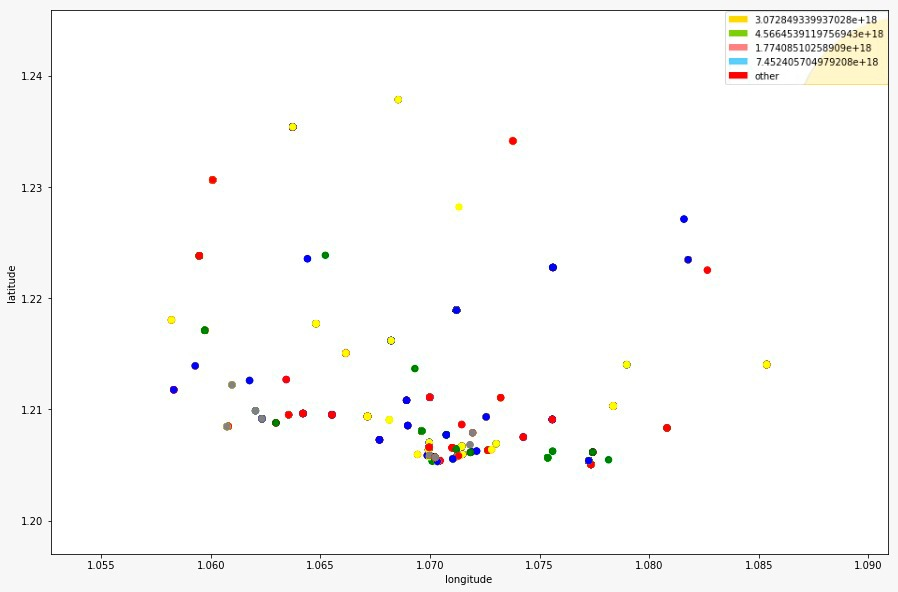
\includegraphics[width=\textwidth]{images/clicks/clicks_lat_long_major_OS.png}
			\caption{Latitud y longitud del click de los dispositivos con distintos os\_major}
		\end{figure}
		\FloatBarrier

		 No se observa que haya una concentracion de algún tipo de dispositivo con la mayor versión de sistema operativo en ningun lugar. De hecho, estan bastantes repartidos.

	\subsubsection{Clicks en la pantalla del dispositivo}

		 Los siguientes gráficos muestran en que posición del celular se realiza el click

		\FloatBarrier
		\begin{figure}[h]
			\centering
			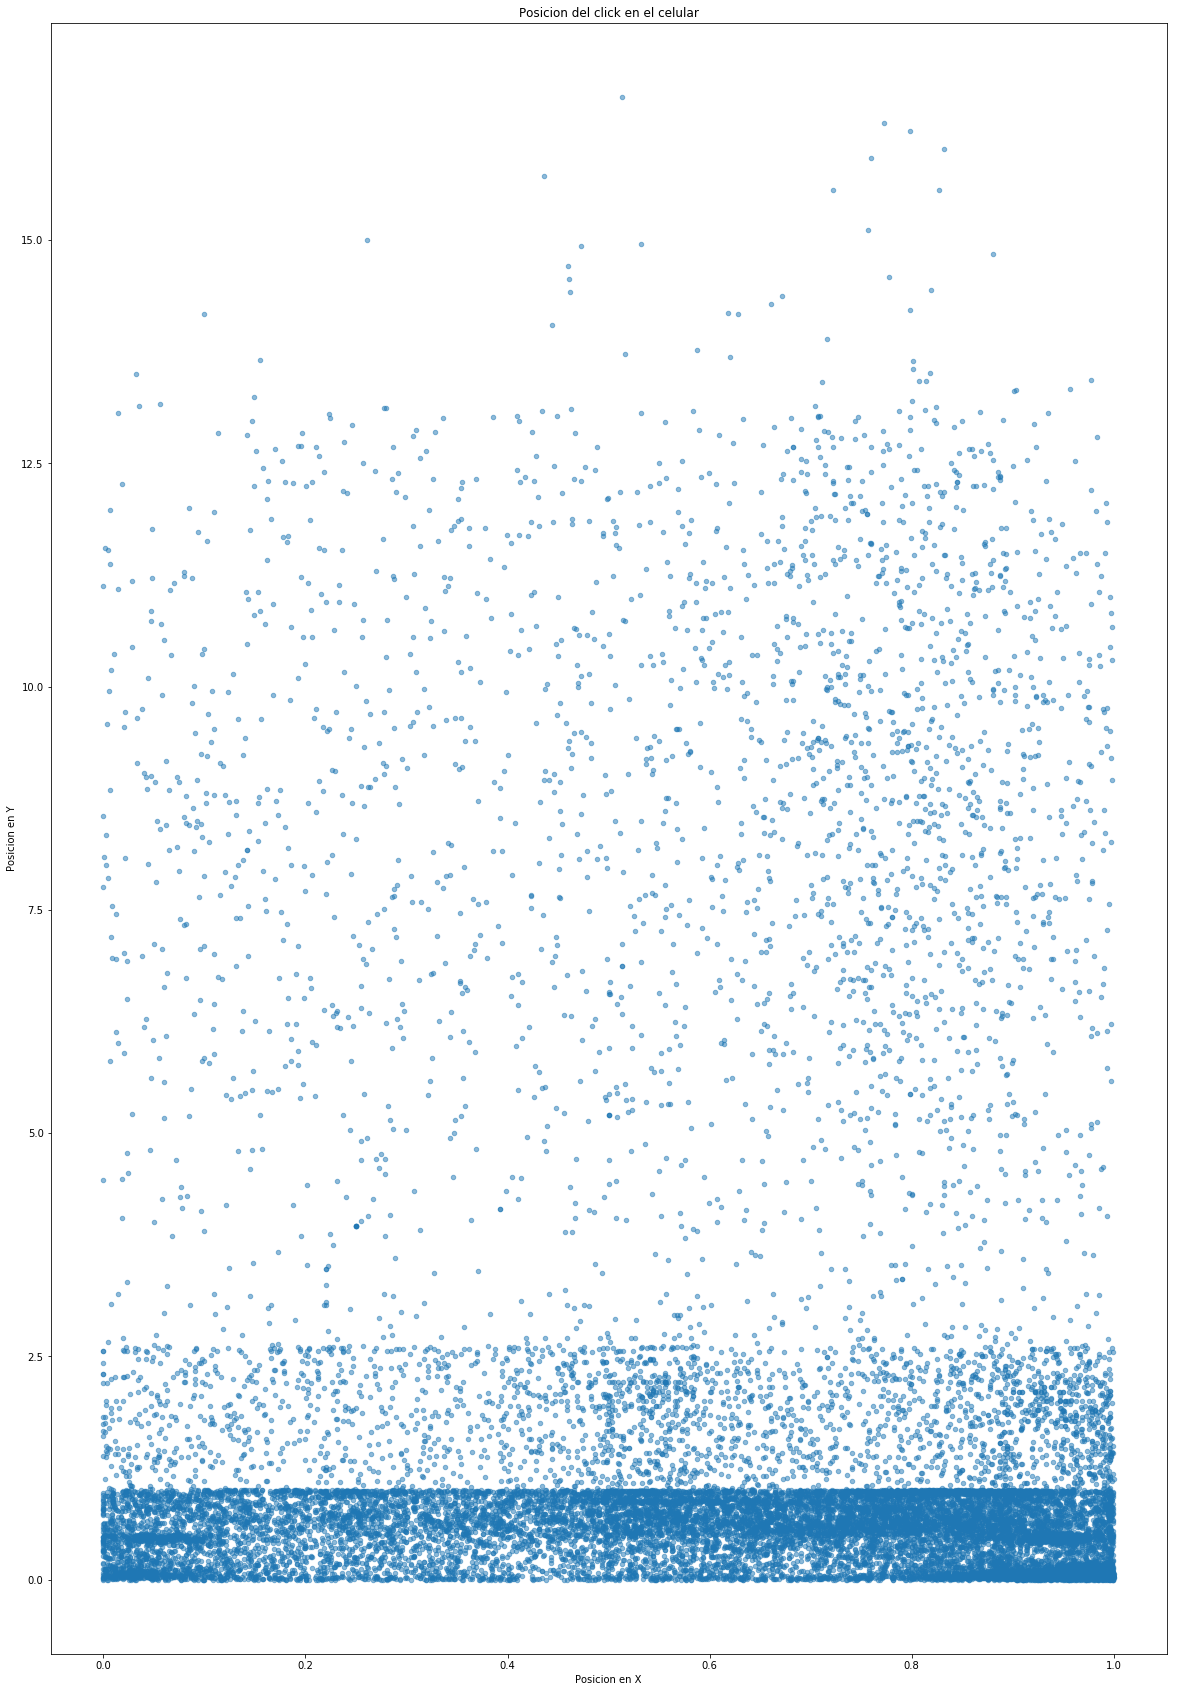
\includegraphics[scale=0.2]{images/clicks/clicks_touch_scatter.png}
			\caption{Posicion del click en pantalla}
		\end{figure}
		\FloatBarrier


		 Se puede ver claramente que la mayor cantidad de clicks se concentra en la parte inferior del teléfono y
		mayormente, en la parte inferior derecha.


	\subsubsection{Tiempo en realizar el click}
 
		 Se nos ocurrió analizar el promedio de tiempo que tarda una persona en realizar click. Primero decidimos filtrar los clicks en el que la persona tardaba más de 10 minutos en hacer click. Esto lo hicimos debido a que había clicks que tardaban más de un año en realizarse y supusimos que es un error en los datos. Llegamos a que una persona tarda 55.5921630859375 segundos en promedio en tocar el anuncio.

	
		 En los siguietes gráficos se mostrará la distribución en el tiempo que tardan los distintos advertiser\_id en hacer click.

		\FloatBarrier
		\begin{figure}[h]
			\centering
			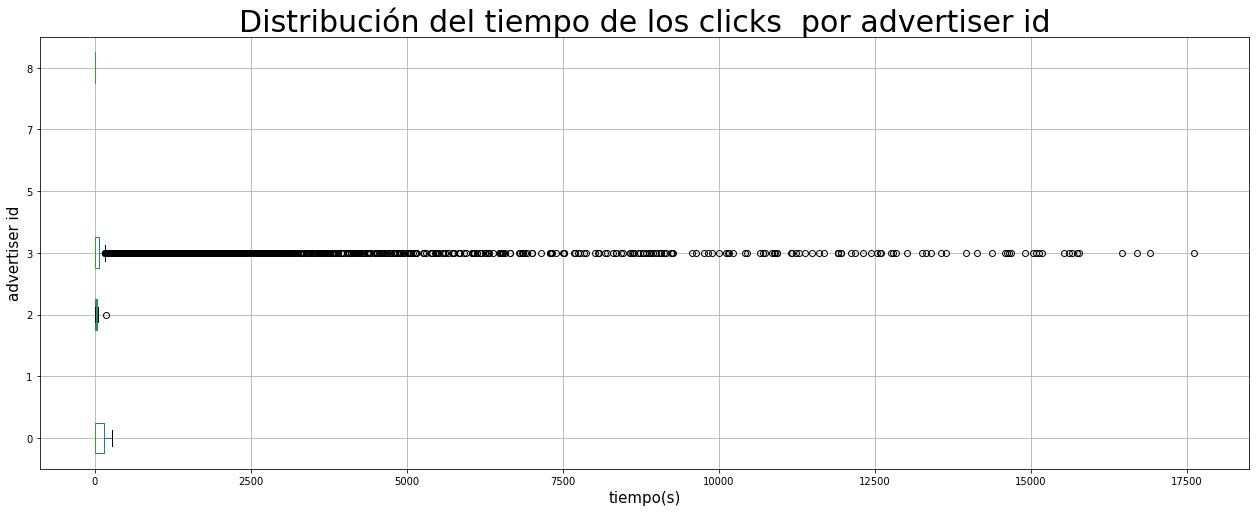
\includegraphics[width=\textwidth]{images/clicks/clicks_advertiser_id_timeToTouch.png}
			\caption{Clicks en el tiempo de los advertiser\_id}
		\end{figure}
		\FloatBarrier


		 Se observa que la mayoría de clicks se realizan en los primeros segundos y practicamente todos por el advertiser\_id 3. Esto es algo totalmente esperable debido a lo que se analizó previamente.
		\newline
		\newline
		 En el siguiete gráfico se mostrará la distribución en el tiempo que tardan los distintos spec\_brands en hacer click.

		\FloatBarrier
		\begin{figure}[h]
			\centering
			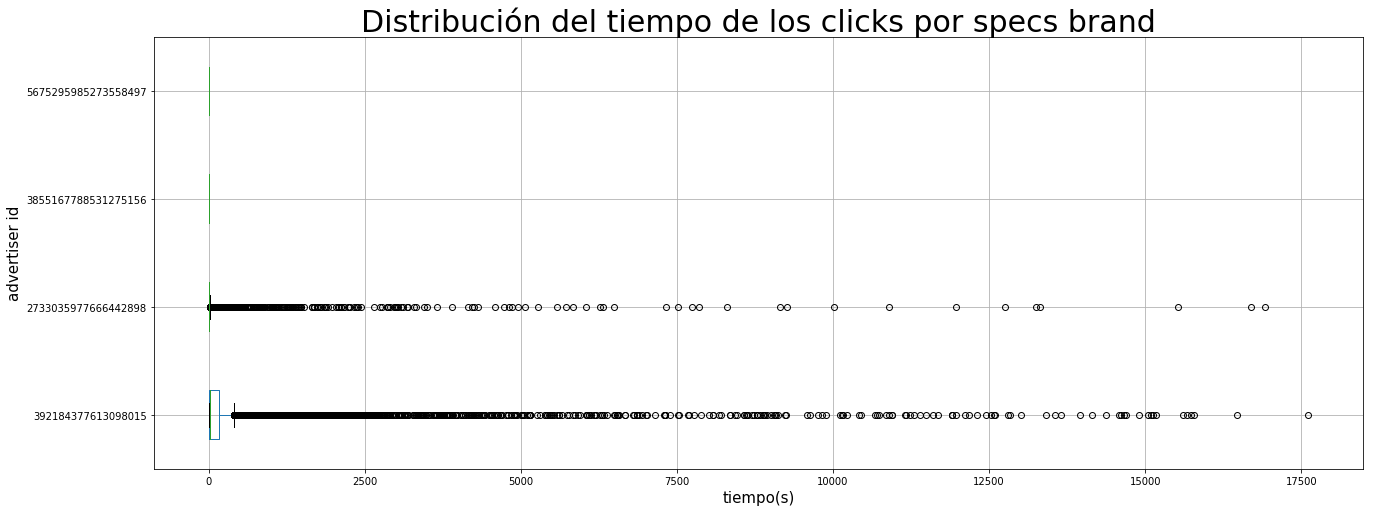
\includegraphics[width=\textwidth]{images/clicks/clicks_specs_brand_timeToTouch.png}
			\caption{Clicks en el tiempo de los spec\_brands}
		\end{figure}
		\FloatBarrier

		 El siguiete gráfico nos muestra la distribución en el tiempo que tardan los distitos sistemas operativos en hacer click.

		\FloatBarrier
		\begin{figure}[h]
			\centering
			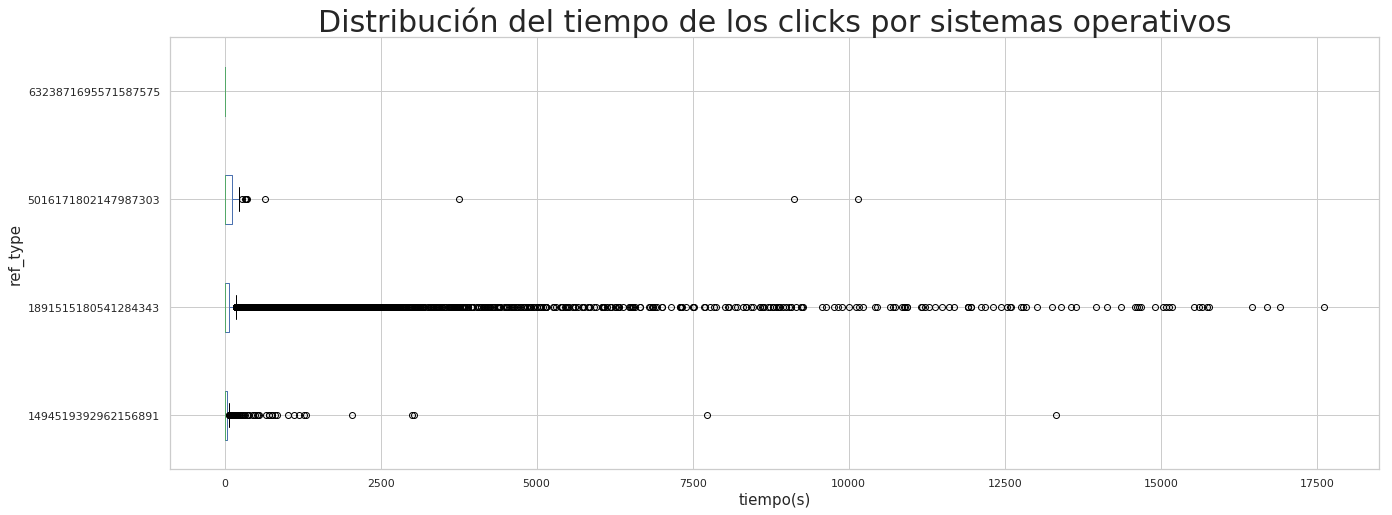
\includegraphics[width=\textwidth]{images/clicks/clicks_ref_type_timeToTouch.png}
			\caption{Clicks en el tiempo de los sistemas opertativos}
		\end{figure}
		\FloatBarrier

		 Se observa lo normal, en ambos sistemas operativos los clicks se concentran en los primeros segundos y luego se van diluyendo con el tiempo. Igualmente se puede notar que el sistema operativo que más clicks tiene, tiene clicks que tardaron bastante en hacerse.




		

\clearpage
\subsection{Eventos}
	\subsubsection{Introducción}
		Los datos sobre eventos se encontraron en el archivo \texttt{events.csv.gzip}, que contenía información sobre los eventos registrados entre el 5/3/19 y el 13/3/19. Esta información incluía el tipo y la fecha del evento, la aplicación que lo generó, datos sobre el dispositivo y sobre el tipo de conexión e información sobre el user agent. A su vez, se tomó la decisión de descartar columnas como el id del dispositivo, el id del evento, la información del país y el id de la transacción, ya que no aportaban información relevante a este análisis.
		
	\subsubsection{Eventos por fecha y hora}
		
		Lo primero que analizaremos será cómo se distribuyeron los eventos cronológicamente, para eso los siguientes gráficos nos muestran esa información de formas distintas.
		
		\FloatBarrier
		\begin{figure}[h]
			\centering
			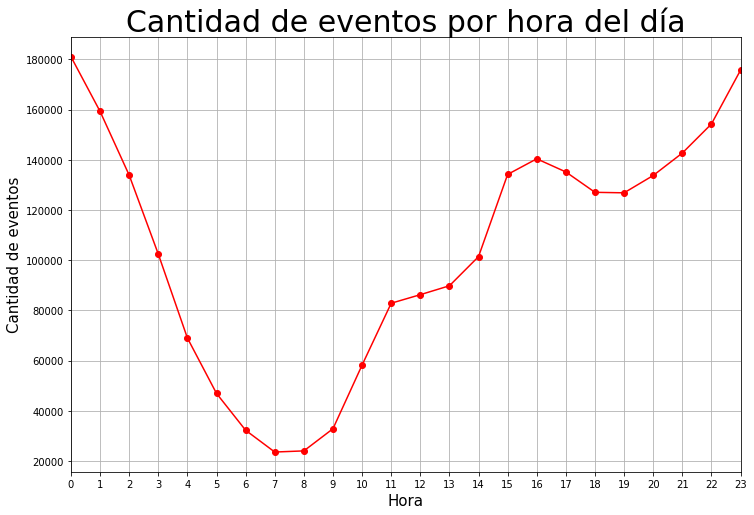
\includegraphics[width=\textwidth]{images/events/eventsxhora.png}
			\caption{Cantidad de eventos por hora del día}
		\end{figure}
		\FloatBarrier
		
		Como se aprecia, se registra una mayor cantidad de eventos en horas de la noche/madrugada y un mínimo absoluto en horas de la mañana. Sin embargo, es de destacar el pico y posterior descenso en horas de la tarde, ya que los valores de las 16 superan incluso a los de horas normalmente no laborables, como las 19 o 20.
		Añadamos ahora a este análisis la fecha de los eventos.
		
		\FloatBarrier
		\begin{figure}[h]
			\centering
			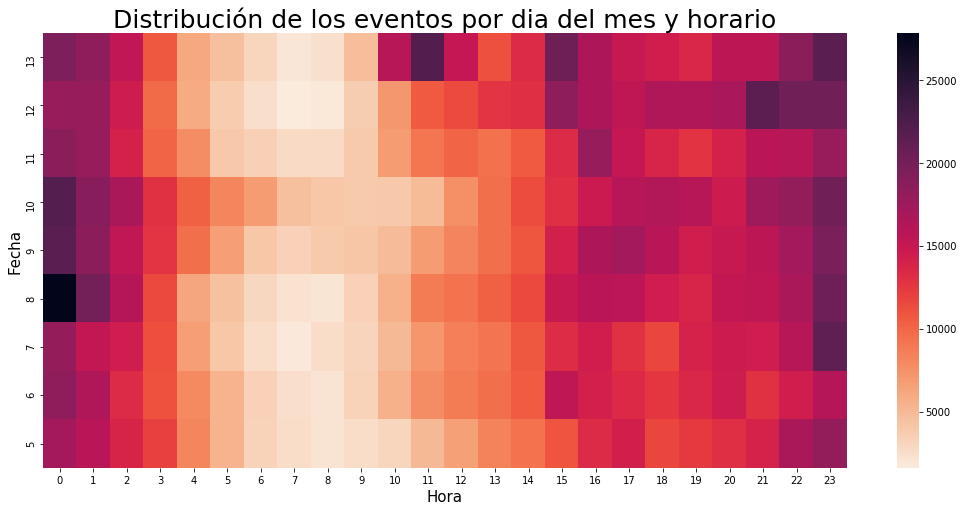
\includegraphics[width=\textwidth]{images/events/eventsxdiayhora.png}
			\caption{Cantidad de eventos por fecha y hora del día}
		\end{figure}
		\FloatBarrier
		
		En la figura se puede apreciar claramente el valle de las horas de la mañana, pero además se ve que el día con más eventos fue el 13, con un llamativo pico a las 11 a.m., mientras que el día 5 fue el de menos ocurrencias. El máximo número de eventos, sin embargo, se registró a comienzos del día 8 y el gráfico muestra un notorio corrimiento de la franja para el 9 y 10 de Marzo, lo que tiene sentido ya que son los días del fin de semana.
		
		Si quisiéramos ver la distribución por días de la semana, primero debemos tener en cuenta que contamos con días repetidos, por lo que será necesario utilizar el promedio.

		\textbf{Aclaración:} Para calcular el promedio, identificamos aquellos días que se repiten, como sabemos que se repiten solo dos veces cada día repetido,
		y que estos días también coinciden con ser los únicos que tienen más de 40.000 filas, calculamos el promedio dividiendo
		por 2 aquellos días que cumplen esta condición. Sin este análisis previo, calcular el promedio hubiese requerido un poco
		 más de trabajo.

		\FloatBarrier
		\begin{figure}[h]
			\centering
			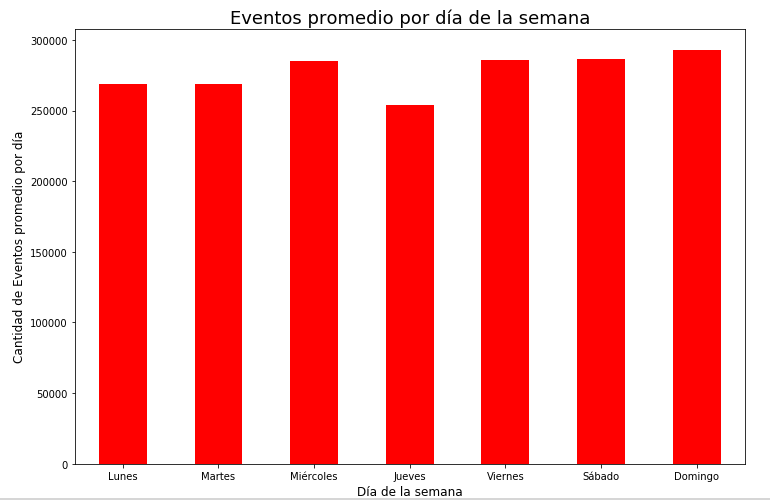
\includegraphics[width=\textwidth]{images/events/eventsxdia.png}
			\caption{Promedio de eventos por día de la semana}
		\end{figure}
		\FloatBarrier
		
		Observamos que es bastante pareja, con un leve aumento los domingos, el día que menos gente trabaja.
		
	\subsubsection{Eventos por aplicación y detalles de los dispositivos}
	
		Al evaluar la cantidad de eventos por aplicación, se debe tener en cuenta primero que se tienen eventos registrados
		en 269 aplicaciones distintas, por lo que se hace imposible graficarlas todas. Para ello, se decidió tomar las
		diez que mayor cantidad de eventos generaron.
		
		\FloatBarrier
		\begin{figure}[h]
			\centering
			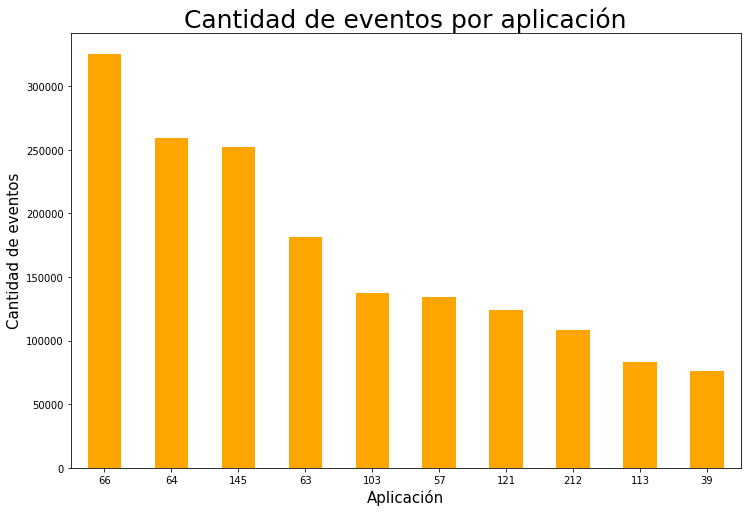
\includegraphics[width=\textwidth]{images/events/evxapp.png}
			\caption{Aplicaciones con mayor cantidad de eventos}
		\end{figure}
		\FloatBarrier
		
		Teniendo éstas, podemos observar, por ejemplo, cuáles son los idiomas predominantes en cada una.
		
		\FloatBarrier
		\begin{figure}[h]
			\centering
			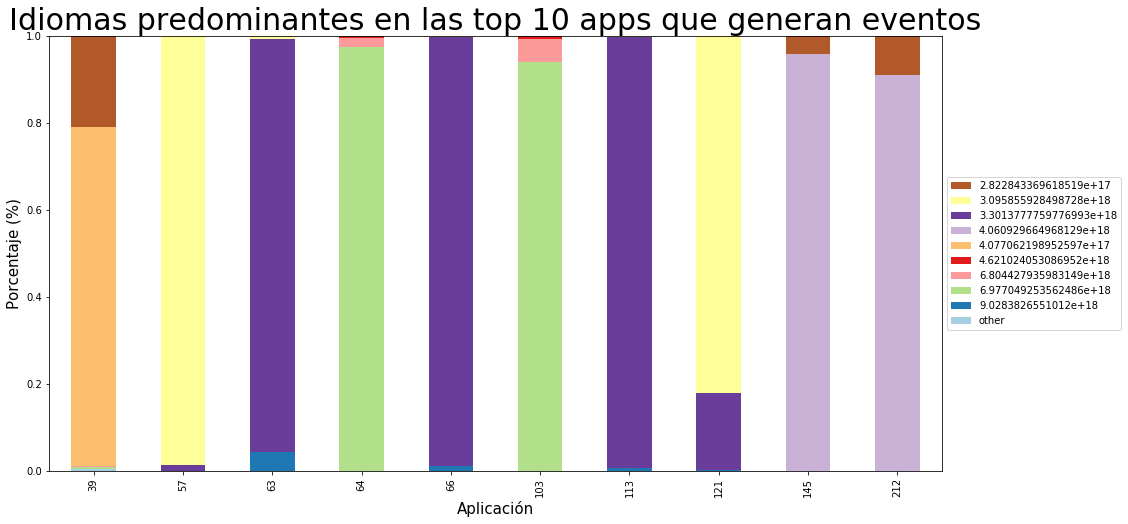
\includegraphics[width=\textwidth]{images/events/idiomasapps.png}
			\caption{Distribución de idiomas para las diez aplicaciones con más eventos}
		\end{figure}
		\FloatBarrier
		
		Como se observa, cada app tiene un idioma que es muy predominante, lo que sugiere que cada una apunta a un público diferente, y cada idioma se distribuye de forma bastante pareja, siendo \texttt{3.3013777759776993e+18} el más utilizado, ya que domina en tres de las diez líderes.
		
		Analicemos ahora el ref type para cada una de las diez.
		
		\FloatBarrier
		\begin{figure}[h]
			\centering
			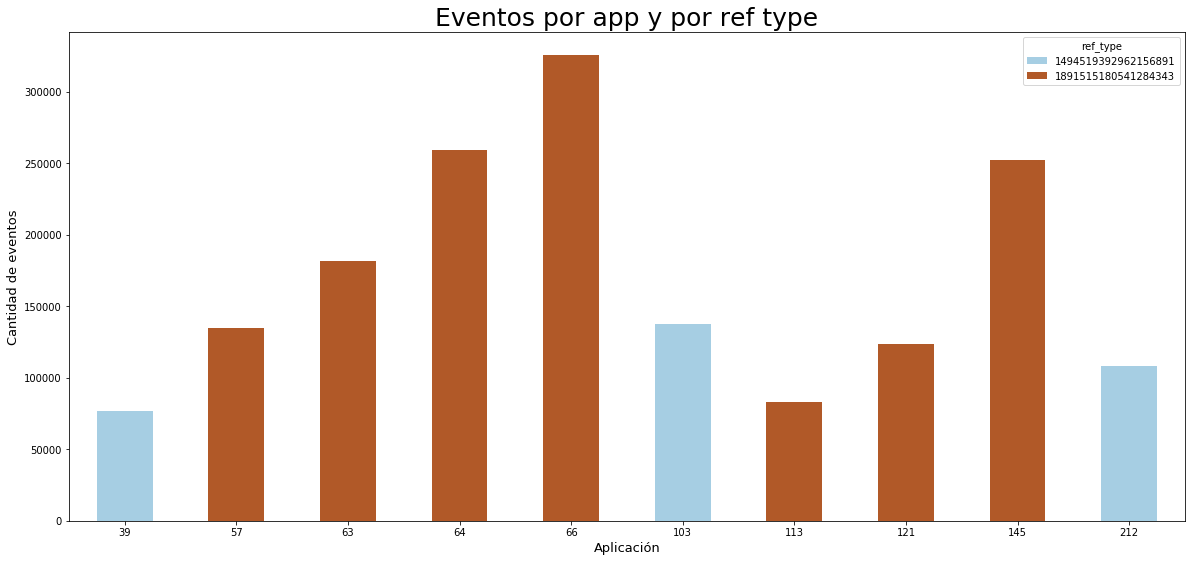
\includegraphics[width=\textwidth]{images/events/evxrf.png}
			\caption{Cantidad de eventos por aplicación del top 10 y ref type}
		\end{figure}
		\FloatBarrier
		
		Como se ve, cada aplicación opera con un solo ref type y el predominante es \texttt{1891515180541284343}.
		
		También se puede analizar qué \textit{session user agent} utiliza cada aplicación.
		
		\FloatBarrier
		\begin{figure}[h]
			\centering
			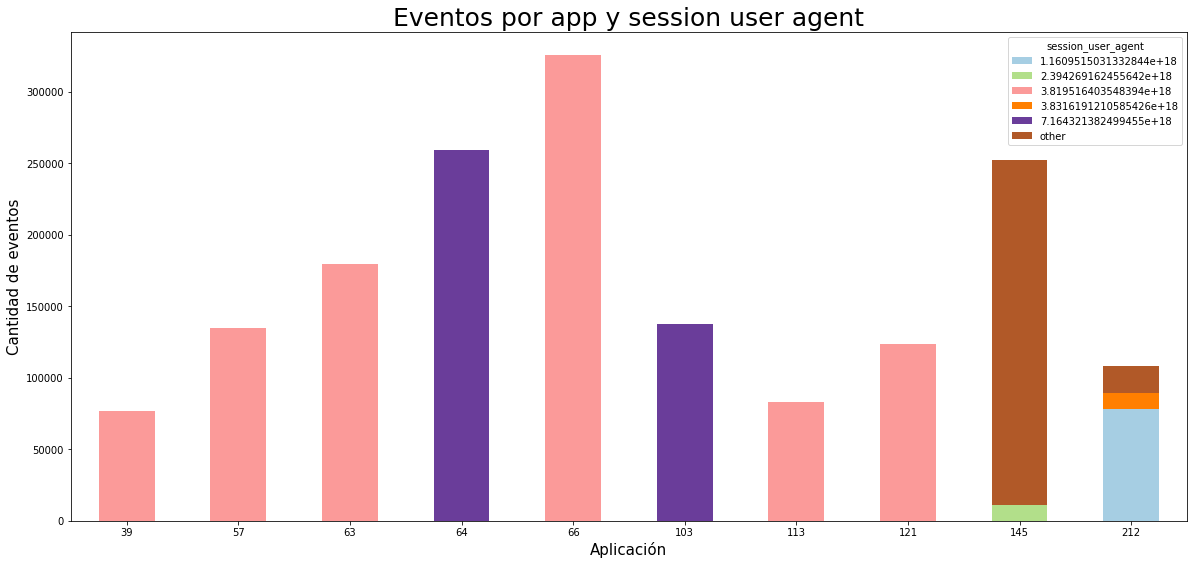
\includegraphics[width=\textwidth]{images/events/evxsua.png}
			\caption{Cantidad de eventos por aplicación del top 10 y session user agent}
		\end{figure}
		\FloatBarrier
		
		A excepción de dos aplicaciones, todas operan con un único session user agent y el que predomina es \texttt{3.819516403548394e+18}, presente en seis. Cabe aclarar que la catgoría \textit{other} está compuesta por 1455 session user agents que aparecían en cantidades muy pequeñas.
		
	\subsubsection{Eventos más frecuentes por tipo}
	
		Otro aspecto interesante a analizar será el tipo de los eventos registrados, el cual nos permite saber cuál era el objetivo del usuario en ese momento. Como se registraron en total 589 tipos distintos de eventos, y como la cantidad de eventos de cada tipo sigue una distribución bastante acorde a la ley de Zipf, se tomarán los primeros diez para este análisis.
		
		\FloatBarrier
		\begin{figure}[h]
			\centering
			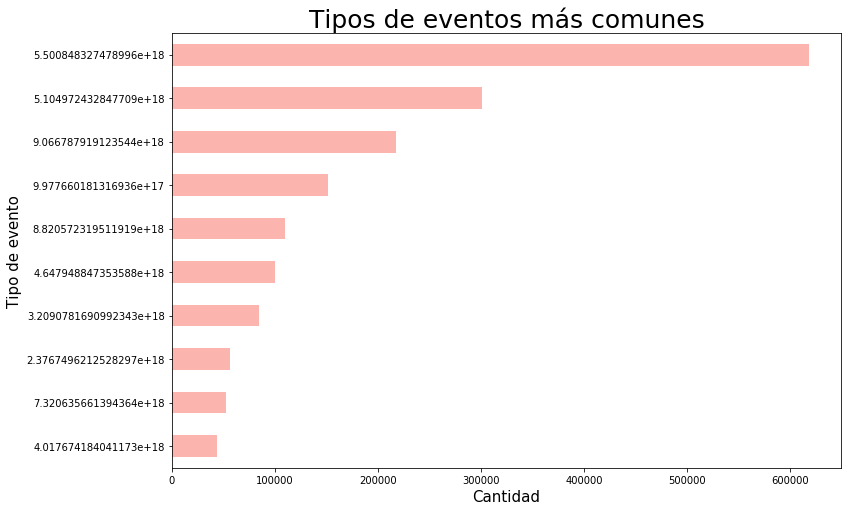
\includegraphics[width=\textwidth]{images/events/top10events.png}
			\caption{Tipos de eventos con más cantidad de apariciones}
		\end{figure}
		\FloatBarrier
		
		Como se puede apreciar, el segundo tipo más común aparece casi exactamente la mitad de las veces que el primero, el tercero casi exactamente un tercio y así sucesivamente, lo que se condice con la ley de Zipf.
		
		Analicemos ahora de dónde provinieron dichos eventos.
		
		\FloatBarrier
		\begin{figure}[h]
			\centering
			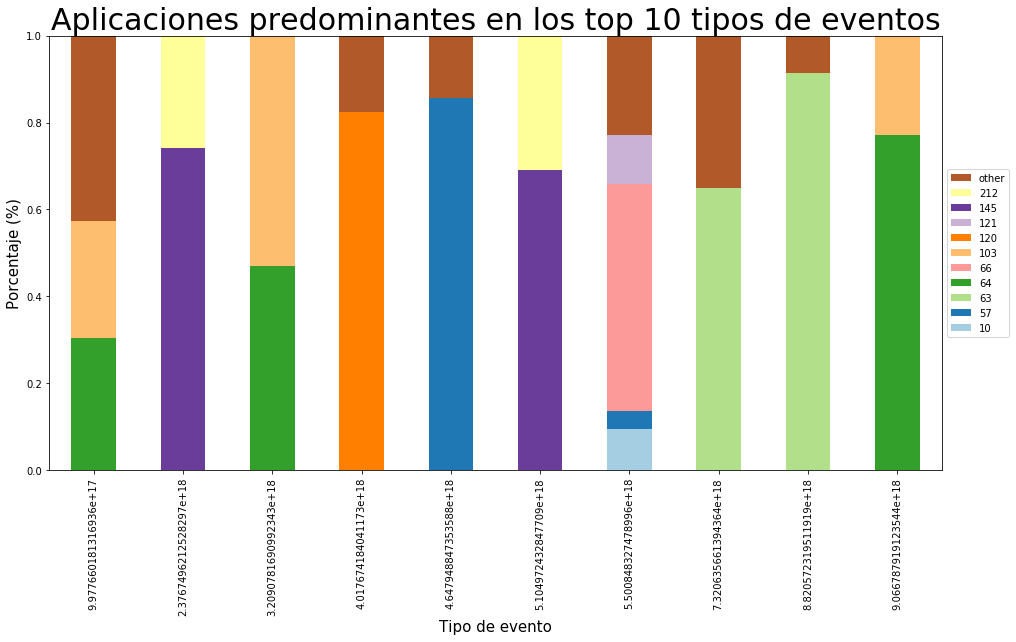
\includegraphics[width=\textwidth]{images/events/appsxev.png}
			\caption{Distribución de las aplicaciones para los diez tipos de evento más comunes}
		\end{figure}
		\FloatBarrier
		
		Podemos también contrastarlos con las aplicaciones que más eventos generan.
		
		\FloatBarrier
		\begin{figure}[h]
			\centering
			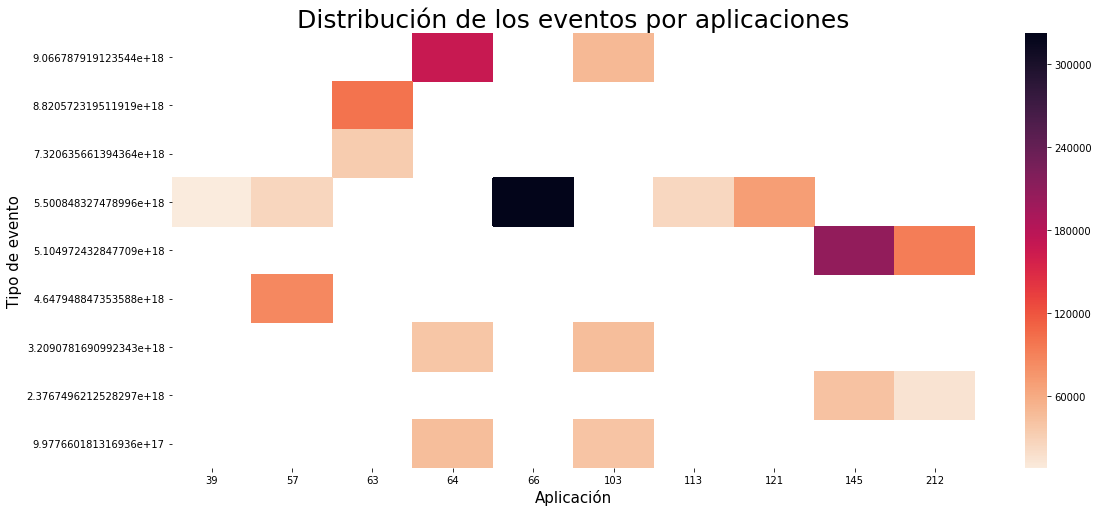
\includegraphics[width=\textwidth]{images/events/top10appsevents.png}
			\caption{Distribución de las diez aplicaciones con más eventos para los diez tipos de evento más comunes}
		\end{figure}
		\FloatBarrier
		
		Como se puede ver, la distribución es bastante heterogénea. Los eventos que genera la app líder son todos del mismo tipo, que a su vez es el tipo de evento más común, por lo que si se busca que los usuarios hagan lo indicado por el evento \texttt{5.500848e+18}, la mejor opción es mostrarles publicidad a través de la app 66. Esto también aplica para las demás, ya que la mayoría solo generan dos o tres tipos de evento distintos y puede utilizarse la misma lógica.
		
	\subsubsection{Eventos por tipo de conexión}
	
		El archivo nos provee con información acerca de la conexión con la que contaban los usuarios a la hora de generar cada evento, ya sea wifi o datos móviles, y en caso de los datos, el tipo de conexión.
	
		En el caso del wifi, vemos que la distribución es la siguiente.
	
		\FloatBarrier
		\begin{figure}[h]
			\centering
			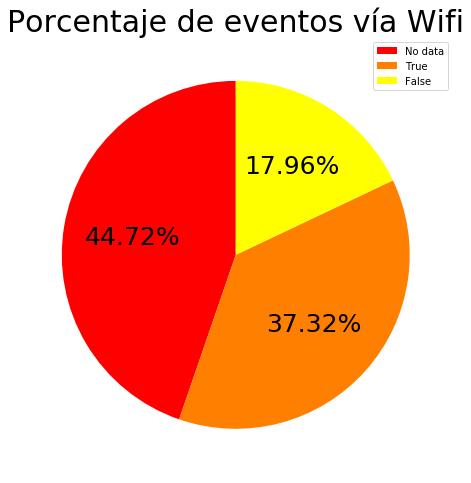
\includegraphics[width=200pt]{images/events/eventosxwifi.png}
			\caption{Distribución de eventos generados vía wifi}
		\end{figure}
		\FloatBarrier
		
		Como se puede observar, no contamos con datos en la mayoría de los eventos, aunque en los que sí se brindan la tendencia es claramente favorable al wifi, como sería esperable.
		
		Sin embargo, para la gran mayoría de los eventos de los que no se tienen datos de conexión wifi sí se tiene información relacionada a conexiones por datos móviles, como la empresa que los provee o el tipo de conexión.
		
		\FloatBarrier
		\begin{figure}[h]
			\centering
			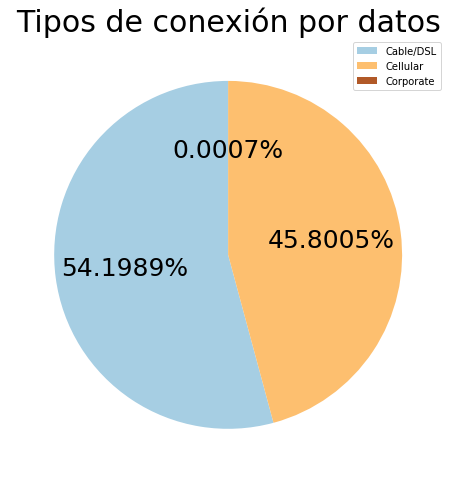
\includegraphics[width=200pt]{images/events/eventsxdatos.png}
			\caption{Tipo de conexión para los eventos generados con datos móviles}
		\end{figure}
		\FloatBarrier
		
		La distribución es pareja con una leve ventaja para las conexiones por cable, mientras que las corporativas son prácticamente despreciables.
		
		Analicemos ahora las empresas que proveen dichas conexiones.
		
		\FloatBarrier
		\begin{figure}[h]
			\centering
			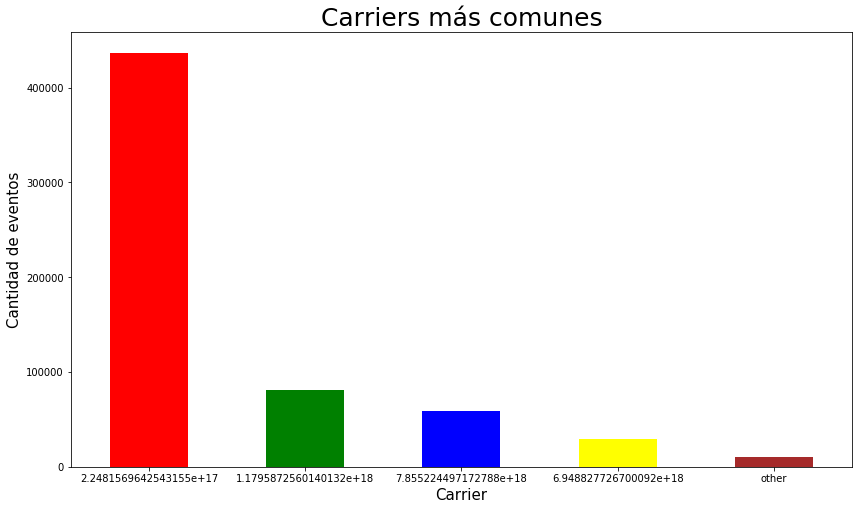
\includegraphics[width=\textwidth]{images/events/carriers.png}
			\caption{Proveedores de servicio más comunes para conexiones por datos móviles}
		\end{figure}
		\FloatBarrier
	
		Se ve que hay un carrier dominante con mucha diferencia con el resto y cabe aclarar que la categoría \textit{other} engloba a 79 carriers distintos con valores muy bajos.
		
		Si combinamos ambos, podemos observar qué tipo de conexión utiliza cada una de las empresas.
		
		\FloatBarrier
		\begin{figure}[h]
			\centering
			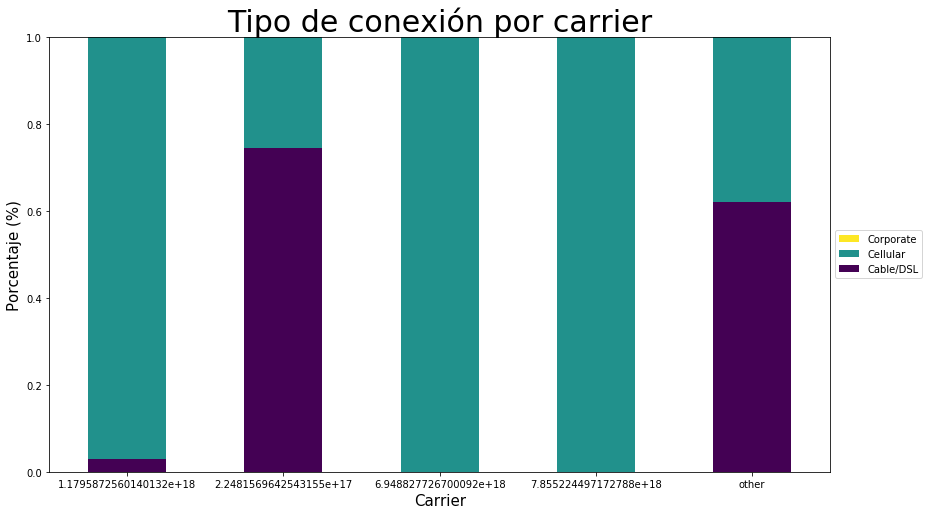
\includegraphics[width=\textwidth]{images/events/carriersxtipo.png}
			\caption{Tipo de conexión por empresa proveedora}
		\end{figure}
		\FloatBarrier
		
		La mayoría usa Cellular mientras que el carrier líder utiliza mayormente Cable/DSL.
		
		\subsubsection*{Eventos más frecuentes para cada tipo de conexión}
			El tipo de conexión con el que se cuenta es un aspecto importante a tener en cuenta a la hora de buscar que los usuarios adopten un comportamiento determinado, por ello analizaremos qué eventos tienden a generarse con los siguientes dos tipos de conexiones.
			\begin{itemize}
				\item \textbf{Wifi}
				\FloatBarrier
				\begin{figure}[h]
					\centering
					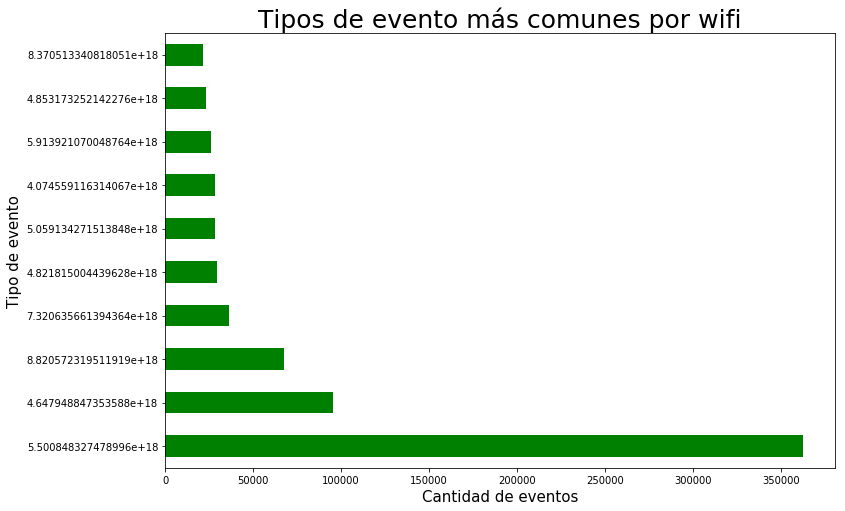
\includegraphics[width=\textwidth]{images/events/eventsxwifi.png}
					\caption{Tipos de evento más frecuentes en conexiones wifi}
				\end{figure}
				\FloatBarrier
				\item \textbf{Datos móviles}
				\FloatBarrier
				\begin{figure}[h]
					\centering
					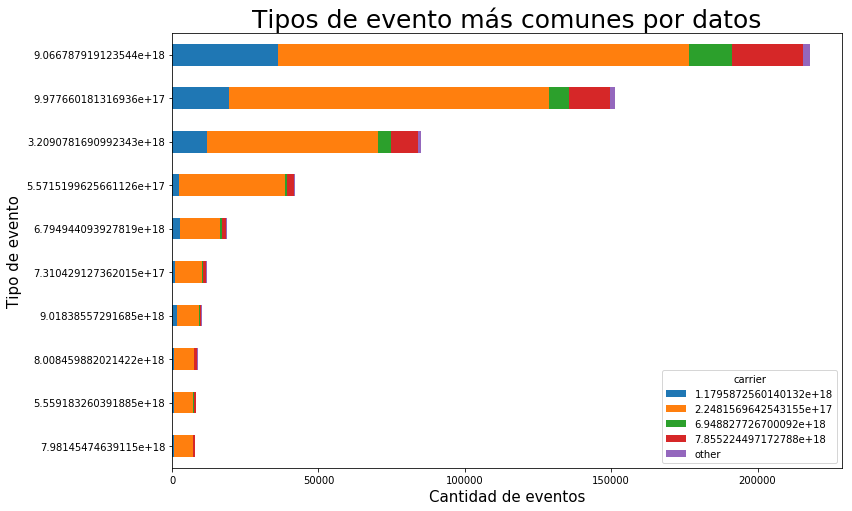
\includegraphics[width=\textwidth]{images/events/eventosxdatosycarrier.png}
					\caption{Tipos de evento más frecuentes para conexiones móviles por carrier}
				\end{figure}
				\FloatBarrier
			\end{itemize}

			Se puede apreciar que cada tipo de conexión genera eventos distintos, por lo que si se quisiera lograr que los usuarios generen el evento \texttt{5.500848327478996e+18}, será importante verificar que cuenten con conexión wifi, mientras que si el que se buscara generar fuera el \texttt{9.066787919123544e+18}, la mejor opción será verificar que estén usando datos móviles y preferiblemete con el carrier \texttt{2.2481569642543155e+17}.

	\subsubsection{Marcas, modelos y eventos}
		Otra cuestión interesante de analizar es el comportamiento de los usuarios de las diferentes marcas de dispositivos. Si bien no contamos con los datos de la marca para todos los eventos, contamos con suficientes datos para evaluar. En ellos encontramos 250 marcas distintas, aunque muchas de ellas de muy bajo impacto. Observemos primero cuáles son las marcas más populares, se muestran las primeras diez, ya que concentran el 94\% de los eventos.

		\FloatBarrier
		\begin{figure}[h]
			\centering
			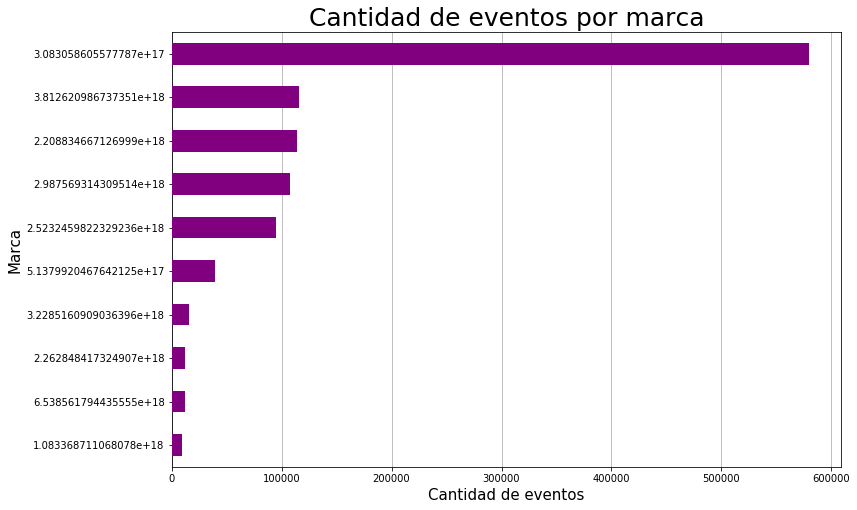
\includegraphics[width=\textwidth]{images/events/marcas.png}
			\caption{Marcas que más eventos generan}
		\end{figure}
		\FloatBarrier

		Se aprecia una notable diferencia entre la marca \texttt{3.083058605577787e+17} y sus competidoras

		Analicemos ahora cómo se relacionan con las aplicaciones.

		\FloatBarrier
		\begin{figure}[h]
			\centering
			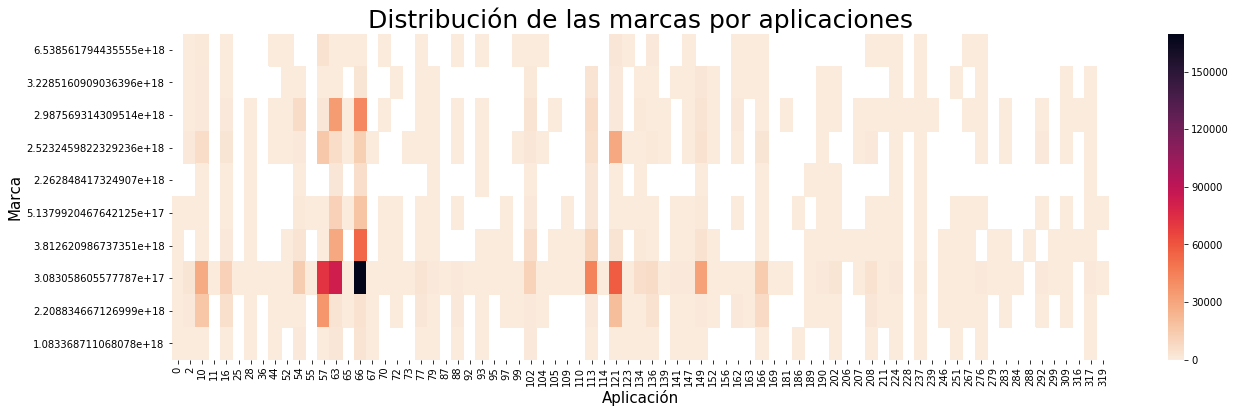
\includegraphics[width=\textwidth]{images/events/brandapps.png}
			\caption{Distribución de aplicaciones por marcas}
		\end{figure}
		\FloatBarrier

		La marca líder tiene fuerte presencia en las aplicaciones 66, 63, 57 y 121, aunque en esta última también influye la marca \texttt{2.5232459822329236e+18}.

	\subsubsection{Ciudades y eventos}
		El lugar de origen de los usuarios de cada evento también será provechoso de analizar para poder distinguir los intereses de los diversos lugares. Si bien en este caso contamos con datos parciales. Lo primero que salta a la vista es que la ciudad \texttt{3.8000799488967747e+18} tiene mucha preponderancia, concentrando el 91,41\% de los eventos. Utilicemos esto para contrastar los eventos más populares y las aplicaciones que más eventos generaron en los distintos lugares, haciendo la distinción entre la ciudad líder y el resto.

		\FloatBarrier
		\begin{figure}[h]
			\centering
			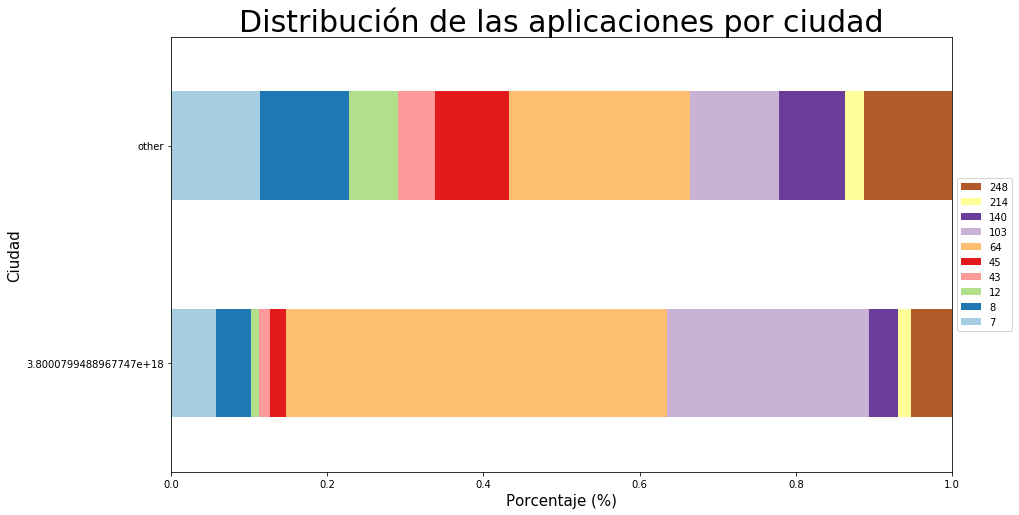
\includegraphics[width=\textwidth]{images/events/citiapp.png}
			\caption{Distribución de aplicaciones por ciudad}
		\end{figure}
		\FloatBarrier

		Notamos que aplicaciones como la 64 y la 103 son mucho más preponderantes en la ciudad \texttt{3.8000799488967747e+18}, mientras que en el resto de lugares, si bien la 64 sigue siendo la más usada, el segundo lugar es mucho más parejo. Esto resulta útil ya que si se quisiera lograr que los usuarios del resto del país generen un evento, será provechoso mostrarles los ads mediante las aplicaciones 64, 8, 7, 248 o 103, cuando si se tratase de la ciudad anterior mencionada la mejor elección sería o la 64 o la 103.
	\subsubsection{Eventos atribuidos a Jampp}
		
\clearpage
\subsection{Instalaciones}
	\subsubsection{Introducción}
		Los datos sobre instalaciones fueron provistos por Jampp en el archivo \texttt{installs.csv.gzip}, el cual contenía información acerca de todas las instalaciones registradas entre los días 5 y 13  Marzo del corriente año, indicando el tipo de aplicaciones descargadas, su fecha de descarga, país de origen, modelo, marca e idioma del dispositivo, entre otras cosas.

		Cabe destacar que se descartaron datos como las direcciones ip y los varios id únicos generados para cada instalación, puesto que no aportaban información relevante al análisis que se pretende hacer en este trabajo, como también los datos del \textit{session user agent}, ya que la misma empresa informó que no los consideran de importancia y pudieron haberse visto modificados por los propios agentes que les proveyeron los datos.

	\subsubsection{Instalaciones por día y hora}
		Para comenzar, lo primero que haremos será ver cómo se distribuyen las instalaciones en el periodo dado.
		\FloatBarrier
		\begin{figure}[h]
			\centering
			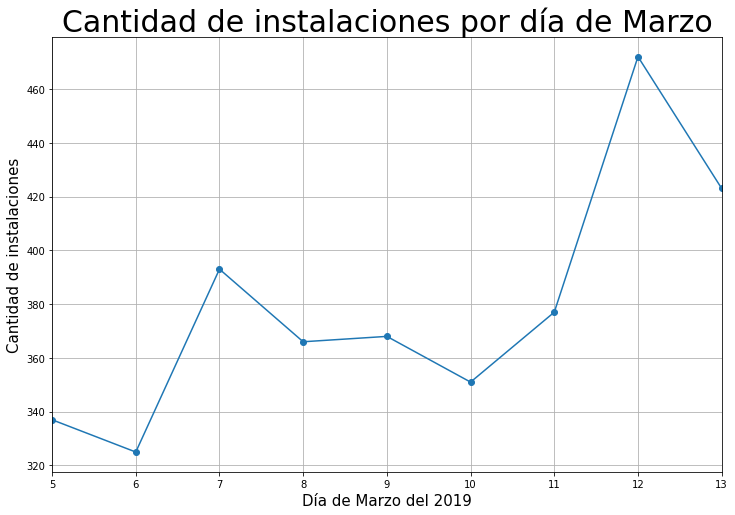
\includegraphics[width=\textwidth]{images/installs/installspordia.png}
			\caption{Instalaciones por día de Marzo}
		\end{figure}
		\FloatBarrier

		Como se puede observar, se registran ascensos considerables entre los días 6 y 7 y 11 y 12, con respectivas caídas al día siguiente, pero manteniendo una tendencia general al alza.

		\FloatBarrier
		\begin{figure}[h]
			\centering
			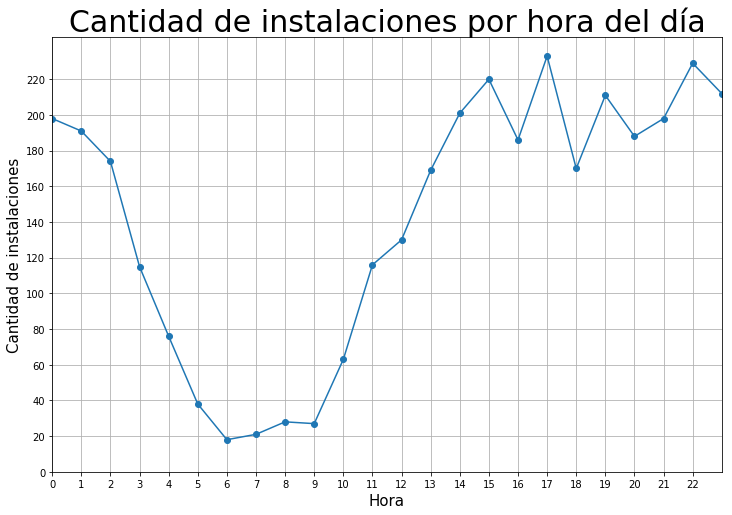
\includegraphics[width=\textwidth]{images/installs/installsxhora.png}
			\caption{Instalaciones por hora del día}
		\end{figure}
		\FloatBarrier

		 El gráfico anterior nos indica que la gran mayoría de las instalaciones se registran en horas de la tarde y la noche, con un pico a las 5 de la tarde. Cabe destacar a su vez el notorio valle que se da en horas de la mañana, donde el número es hasta diez veces menor que en el punto máximo.

		 Para un análisis más general, la siguiente figura engloba los dos puntos mencionados anteriormente.

		\FloatBarrier
		\begin{figure}[h]
			\centering
			\includegraphics[width=\textwidth]{images/installs/heatmapfecha.png}
			\caption{Instalaciones por fecha y hora}
		\end{figure}
		\FloatBarrier

		Se puede observar claramente el valle de las horas de la mañana, como así también el pico que se da en el día 12. Sin embargo, este gráfico resulta útil ya que permite notar que tanto en los días 6 y 13 a las 6 de la mañana, el día 11 a las 7 y el 10 a las 9 no se produjo ninguna instalación.

	\subsubsection{Instalaciones por aplicación} \label{aplicaciones}
		Resultará de utilidad conocer de que aplicación provienen las instalaciones registradas y observar cual es la tendencia en ese aspecto para determinar en cuales es mejor colocar la publicidad.

		\FloatBarrier
		\begin{figure}[h]
			\centering
			\includegraphics[width = \textwidth]{images/installs/aplicacionesvc.png}
			\caption{Instalaciones por aplicación}
		\end{figure}
		\FloatBarrier

		La figura anterior muestra un dominio claro de las aplicaciones 7 y 9 por sobre las demás, ya que la segunda casi duplica en cantidad a la tercera. Además, se puede ver otra diferencia importante{\textemdash}otra vez, de casi el doble{\textemdash}entre la quinta y la sexta, lo que deja en evidencia cuales son las que dominan en este campo, puesto que las primeras cinco aplicaciones concentran más del 80\% de las instalaciones.

	\subsubsection{Instalaciones por fecha según la aplicación}
		A continuación veremos a qué aplicaciones pertenecen las instalaciones según el día y la hora del día, lo que puede servir para determinar en qué momento apostar por una u otra aplicación. Cabe destacar que, para ello se agruparon todas aquellas aplicaciones que generaron un número muy bajo (menos de 90) de instalaciones en la categoría \textit{other}.

		\FloatBarrier
		\begin{figure}[h]
			\centering
			\includegraphics[width= \textwidth]{images/installs/appsxdiaarea.png}
			\caption{Incidencia de las aplicaciones según el día}
		\end{figure}
		\FloatBarrier

		Como se puede observar, la aplicación 7 dominó la mayoría de los días aunque disminuyendo hacia el 12 y el 13, donde fue superada por la 9. La tercera aplicación con más instalaciones, la 10, se mantuvo bastante estable durante los últimos cinco días, mientras que los días 10 y 12 la número 2, de poca preponderancia en otros días, obtuvo su mejor resultado. Cabe aclarar además, que si bien en días como el 9 se ve bastante incidencia de la categoría \textit{other}, ésta engloba los resultados de 23 aplicaciones distintas.

		\FloatBarrier
		\begin{figure}[h]
			\centering
			\includegraphics[width=\textwidth]{images/installs/appsxhora.png}
			\caption{Incidencia de las aplicaciones según la hora del día}
		\end{figure}
		\FloatBarrier

		En cuanto a la hora cabe destacar que la segunda aplicación en instalaciones no tiene presencia algúna a las 8 a.m., que es a su vez el momento del día donde más incidencia tiene una aplicación de poca presencia como la 2. La tendencia sigue mostrando a la número 7 como dominadora absoluta en todos los horarios.

	\subsubsection{Instalaciones por país}
		El país de origen es un aspecto a considerar a la hora de decidir qué advertisers priorizar para cada situación. En este caso Jampp nos provee información de instalaciones en dos países distintos.

		\FloatBarrier
		\begin{figure}[h]
			\centering
			\includegraphics[width=200pt]{images/installs/piechartpaises.png}
			\caption{País de origen de las instalaciones}
		\end{figure}
		\FloatBarrier

		La proporción es bastante pareja, con leve mayoría para el país \texttt{6333597102633388268}.

	\subsubsection{Instalaciones por tipo}
		Los dispositivos se clasifican en dos grandes grupos, aquellos que provienen de Apple y los que provienen de Google.

		\FloatBarrier
		\begin{figure}[h]
			\centering
			\includegraphics[width= 200pt]{images/installs/ref_type.png}
			\caption{Tipo de referencia de las instalaciones}
		\end{figure}
		\FloatBarrier

		Como se observa, el claro dominador es \texttt{1891515180541284343}.

	\subsubsection{Aplicaciones por país y tipo}

		Analicemos ahora de donde provienen las instalaciones de las 5 aplicaciones con más installs.

		\FloatBarrier
		\begin{figure}[h]
			\centering
			\includegraphics[width=\textwidth]{images/installs/appsxpais.png}
			\caption{Distribución de países para las top 5 aplicaciones en instalaciones}
		\end{figure}
		\FloatBarrier

		Sorprendentemente el gráfico es determinante, las aplicaciones provienen o de un país o del otro, ninguna está presente en ambos.

		\FloatBarrier
		\begin{figure}[h]
			\centering
			\includegraphics[width=\textwidth]{images/installs/paisref.png}
			\caption{Distribución de ref types para las top 5 aplicaciones en instalaciones}
		\end{figure}
		\FloatBarrier

		En el caso de los tipos sucede lo mismo, aunque esto es más esperable, ya que existen muchas aplicaciones que son exclusivas de Apple o de Google. Esta información es útil a la hora de determinar el advertiser a seleccionar en cada subasta, ya que la aplicación o servicio a mostrar en la publicidad debe estar disponible para ese tipo.

	\subsubsection{Idiomas y aplicaciones}
		Otro aspecto importante a considerar será el idioma del dispositivo al que se le mostrará la publicidad, ya que el usuario debe entender el mensaje.

		\FloatBarrier
		\begin{figure}[h]
			\centering
			\includegraphics[width=\textwidth]{images/installs/idiomas.png}
			\caption{Idioma de entrada con mayor número de instalaciones}
		\end{figure}
		\FloatBarrier

		Vemos que hay un idioma claramente predominante, luego dos en nivel parejo y una brecha considerable.
		Por esta razón, y para mayor simplicidad de los gráficos, se agruparán los 26 idiomas menos predominantes en la categoría \textit{other}.

		Analicemos ahora como se distribuyen los idiomas en las 5 applicaciones más instaladas.

		\FloatBarrier
		\begin{figure}[h]
			\centering
			\includegraphics[width=\textwidth]{images/installs/idiomasapps.png}
			\caption{Idioma de entrada de los dispositivos para las 5 aplicaciones líderes en instalaciones}
		\end{figure}
		\FloatBarrier

		Como se puede ver, las aplicaciones líderes (7 y 9 respectivamente) se utilizan con idiomas distintos, mientras que en 10 y 16 predominan otros dos lenguajes diferentes.

	\subsubsection{Instalaciones por marca}

		La información de marca y modelo de los dispositivos que instalaron ........

		\FloatBarrier
		\begin{figure}[h]
			\centering
			\includegraphics[width=\textwidth]{images/installs/marcas.png}
			\caption{Marcas con más instalaciones}
		\end{figure}
		\FloatBarrier

		Como se aprecia, hay una marca que lidera absolutamente con una cantidad de installs dos veces y media mayor a su inmediata competidora.

		Lo interesante será conocer además el tipo de dispositivo que producen esas marcas, para así determinar el tipo de publicidades que soportarán y así elegir mejor al advertiser.

		Del gráfico vemos que todas las marcas de las que se tiene registro utilizan el tipo \texttt{1891515180541284343} a excpción de una, la \texttt{5.951324980112395e+18}, que utiliza el otro.

	\subsubsection{Instalaciones wifi y user agents}

		Otro aspecto a considerar es la conexión con la que cuentan los usuarios al momento de decidir si hacer caso o no a algúna publicidad. Los datos que nos proporciona Jampp nos indican si las instalaciones fueron hechas vía conexión wifi.

		Inicialmente se esperaría que sea mayor el número de instalaciones vía wifi, ya que los datos móviles suelen tener un límite de uso bastante bajo.

		\FloatBarrier
		\begin{figure}[h]
			\centering
			\includegraphics[width=200pt]{images/installs/Wifi.png}
			\caption{Instalaciones por conexión wifi.}
		\end{figure}
		\FloatBarrier

		Sorprendentemente la figura muestra que para una gran mayoría de las instalaciones no se proporcionó data respecto de la conexión. Sin embargo, y en concordancia con lo mencionado previamente, en los casos en los que sí se tiene información resulta claro ver que la mayor parte de dichas instalaciones sí fueron realizadas vía conexión wifi.

		Trasladando estos datos a las aplicaciones vemos.

		\FloatBarrier
		\begin{figure}[h]
			\centering
			\includegraphics[width=\textwidth]{images/installs/appswifi.png}
			\caption{Instalaciones por conexión wifi según la aplicación.}
		\end{figure}
		\FloatBarrier

		Lo primero que observamos es que la cantidad de aplicaciones de las que se tienen datos de conexión es reducida en comparación al total, ya que , por ejemplo, la aplicación líder en instalaciones no especifica tipo de conexión en ninguna de sus installs. Sin embargo, de este gráfico puede tomarse el hecho de que, si bien la tendencia indica que la mayoría de las instalaciones de las que se tienen datos se realizaron vía wifi, hay aplicaciones como 21 ,donde la proporción es más pareja, o la 36, donde se invierte. Esto puede servir para determinar qué tipo de publicidad mostrar, puesto que en los casos donde no se cuenta con wifi hay que tener en cuenta el consumo, para no gastarle los datos al usuario.


		Por otra parte, el hecho de que un install se haya realizado por wifi nos permite conocer otro dato importante, el \textit{user agent} relacionado a la acción.

		Análogamente a lo hecho al comienzo de la sección \ref{aplicaciones}, se analizaron los user agents.

		\FloatBarrier
		\begin{figure}[h]
			\centering
			\includegraphics[width=\textwidth]{images/installs/useragents.png}
			\caption{User agents por instalaciones}
		\end{figure}
		\FloatBarrier

		Resulta evidente que los dominadores absolutos de la categoría son Dalvik y MercadoPago, con agentes casi sin presencia, como Mozilla y takealot, que cuentan sólamente con una instalación.

		\subsubsection{Instalaciones atribuidas a Jampp}
		Será de particular importancia saber cuantas de las instalaciones se le atribuyeron oficialmente a Jampp, es decir, cuantas de ellas fueron realmente obra de la empresa. Los datos proporcionados hacen dos tipos de distinciones.

		\FloatBarrier
		\begin{itemize}
		\item \textbf{Attributed}: Indica si la instalación le fue reconocida oficialmente a Jampp.
		\item \textbf{Implicit}: Indica si la instalación se registró de manera implícita, es decir, se realizó por otro canal.
		\end{itemize}
		\FloatBarrier

		En este aspecto, los datos indican que absolutamente ninguna de las instalaciones le fue atribuida a Jampp, lo que indica un porcentaje de efectividad del 0\%. Sin embargo, para la categoría \textit{implicit}, los resultados fueron los siguientes.

		\FloatBarrier
		\begin{figure}[h]
			\centering
			\includegraphics[width=300pt]{images/installs/implicit.png}
			\caption{Porcentaje de instalaciones registradas por un canal distinto a Jampp}
		\end{figure}
		\FloatBarrier

		Los datos muestran un \textit{ratio} de algo más de 1 de cada 4 instalaciones se realizaron por fuera de la influencia de Jampp.

		Si lo trasladamos nuevamente a las 5 aplicaciones más instaladas.

		\FloatBarrier
		\begin{figure}[h]
			\centering
			\includegraphics[width=\textwidth]{images/installs/incidenciacomp.png}
			\caption{Porcentaje de instalaciones por algún otro método para las top 5 apps en descargas}
		\end{figure}
		\FloatBarrier

		Como podemos ver, los resultados van acorde a lo mostrado en la figura anterior, con casos como el de la aplicación 10, donde casi el 40\% de las instalaciones son externas. Sin embargo, cabe destacar que en la aplicación líder en descargas, la cual supera a su perseguidora por más de 200 instalaciones (véase sección \ref{aplicaciones}), es donde estos métodos tienen menos presencia.

\clearpage
\section{Análisis de archivos en conjunto}
\subsection{Clicks y subastas}
	\subsubsection{Análisis general}
	 Hay dos temas que se van a analizar en estos dos archivos en conjunto:
	\begin{enumerate}
		\item Relación entre cantidades de clicks y de subastas.
		\item Advertisers
	\end{enumerate}

	 Empezamos mostrando gráficos representativos de los datos.
	\FloatBarrier
		\begin{figure}[h]
			\centering
			\includegraphics[width=350pt]{images/auctions-clicks/subastasterminadasenclicks.png}
			\caption{Relación clicks/subastas}
			\label{subastasterminadasenclicks}
		\end{figure}

		\begin{figure}[h]
			\centering
			\includegraphics[width=350pt]{images/auctions-clicks/subyclickspordia.png}
			\caption{Cantidad de clicks y subastas por día}
			\label{clicksysubastaspordia}
		\end{figure}

		\begin{figure}[h]
			\centering
			\includegraphics[width=350pt]{images/auctions-clicks/relauctionsclickspordia.png}
			\caption{Relación clicks/subastas por día}
			\label{relclickssubastas}
		\end{figure}
	\FloatBarrier

	 Podemos obtener conclusiones importantes en base a estos gráficos, teniendo en cuenta que cuando se habla de relación clicks/subastas o de subastas que terminan en clicks no se hace referencia a subastas, o clicks, individuales sino a una relación en conjunto, ya que no podemos identificar qupe subasta termino en cada click. Por lo tanto cuando digamos relación clicks/subastas estaremos hablando de $\frac{n_{clicks}}{n_{subastas}}$, siendo $n_{clicks}$ la cantidad de clicks y $n_{subastas}$ la cantidad de subastas.
	\begin{itemize}
		\item La cantidad de clicks es ínfima en relación a la cantidad de subastas. Se pueden perder cantidades en dos partes del proceso (pocas subastas se ganan  y/o poca gente hace clicks una vez que se gana la subasta y se muestra un anuncio). Gráfico \ref{subastasterminadasenclicks}.
		\item No tiene mucho sentido el gráfico \ref{clicksysubastaspordia} ya que la cantidad de subastas es tan grande en comparación con la cantidad de clicks que la figura de clicks se achata cercana a cero.
		\item El gráfico \ref{relclickssubastas} nos permite ver mejor lo confirmado en el ítem anterior. Día a día la relación $\frac{n_{clicks}}{n_{subastas}}$ es menor al 0,005%.
	\end{itemize}

	 Por otra parte, vimos en la sección "Subastas" que cada device\_id tenía asociado una plataforma. Los datos obtenidos nos permiten saber quién es el advertiser predominante en cada plataforma. Para ello vemos dos gráficos (uno para la plataforma '1' y otro para la plataforma '2').

	\FloatBarrier
		\begin{figure}[h]
			\centering
			\includegraphics[width=350pt]{images/auctions-clicks/advporSO.png}
			\caption{Cantidad de clicks en dispositivos con plataforma '1' para cada advertiser}
			\label{advporSO}
		\end{figure}

		\begin{figure}[h]
			\centering
			\includegraphics[width=350pt]{images/auctions-clicks/advporSO2.png}
			\caption{Cantidad de clicks en dispositivos con plataforma '2' para cada advertiser}
			\label{advporSO2}
		\end{figure}
	\FloatBarrier

	 Se puede ver, claramente, que el advertiser '3' es predominante para ambas plataformas. Pero además, un dato interesante es la diferencia en la cantidad de clicks entre las plataformas. Cerca de 25000 para la plataforma '1' y cerca de 700 para la plataforma '2' (en el anexo 'tablas de datos' se podrán comprobar los numeros exactos). Esta diferencia entre los sistemas operativos ya la habíamso visto en la seccion "Subastas".



\section{Conclusión}

\clearpage
\appendix
\section{Tablas de datos}
	\subsection{Subastas}
	\begin{center}
	\begin{tabular}{ |c|c| }
    	\hline
        Día de Marzo & Cantidad de subastas \\
        \hline\hline
		5 & 1182401\\
        \hline
       	6 & 1032970 \\
        \hline
        7 & 2047661 \\
        \hline
        8 & 2303002 \\
        \hline
        9 & 2074552\\
        \hline
       	10 & 2637534 \\
        \hline
        11 & 2574916 \\
        \hline
        12 & 2779910 \\
        \hline
        13 & 2938373\\
        \hline
	\end{tabular}
	

		
	\begin{tabular}{ |c|c|c| }
    	\hline
        Día de Marzo & Plataforma & Cantidad de subastas \\
        \hline\hline
		5	& 1 & 719286 \\
			& 2	& 463115 \\
        \hline
       	6	& 1 & 579624 \\
			& 2	& 453346 \\
        \hline
        7	& 1 & 1617609 \\
			& 2	& 430052 \\
        \hline
        8	& 1 & 1898054 \\
			& 2	& 404948 \\
        \hline
        9	& 1 & 1618742 \\
			& 2	& 455810 \\
        \hline
       	10	& 1 & 2149876 \\
			& 2	& 487658 \\
        \hline
       	11	& 1 & 2165005 \\
			& 2	& 409911 \\
        \hline
        12	& 1 & 2337162 \\
			& 2	& 442748 \\
		\hline
       	13	& 1 & 2456467 \\
			& 2	& 481906 \\
        \hline
	\end{tabular}
	
	\begin{tabular}{ |c|c| }
    	\hline
        Hora del día & Cantidad de subastas \\
        \hline\hline
		0 & 1005716\\
        \hline
       	1 & 1371091 \\
        \hline
        2 & 1388464 \\
        \hline
        3 & 1027541 \\
        \hline
        4 & 716194\\
        \hline
       	5 & 487243 \\
        \hline
        6 & 325730 \\
        \hline
        7 & 245109 \\
        \hline
        8 & 247915\\
        \hline
        9 & 329604\\
        \hline
       	10 & 494726 \\
        \hline
        11 & 627907 \\
        \hline
        12 & 748935 \\
        \hline
        13 & 741996\\
        \hline
       	14 & 805579 \\
        \hline
        15 & 883824 \\
        \hline
        16 & 941866 \\
        \hline
        17 & 967539\\
        \hline
        18 & 989528 \\
        \hline
        19 & 994381\\
        \hline
       	20 & 933318 \\
        \hline
        21 & 1015053 \\
        \hline
        22 & 1108219 \\
        \hline
        23 & 1173841\\
        \hline
	\end{tabular}
 	
 	\begin{tabular}{ |c|c|c| }
    	\hline
        Hora del día & Plataforma & Cantidad de subastas \\
        \hline\hline
		0	&	1	&	755945 \\
			&	2 	&	249771 \\
		\hline
		1 	&	1	& 	1085385 \\
			&	2	& 	285706 \\
		\hline
		2 	&	1	& 	1123515 \\
			&	2	& 	264949 \\
		\hline
		3 	&	1	& 	829257 \\
			&	2	& 	198284 \\
		\hline
		4 	&	1	& 	572832 \\
			&	2	& 	143362 \\
		\hline
		5 	&	1	& 	390653 \\
			&	2	& 	96590 \\
		\hline
		6 	&	1	& 	260795 \\
			&	2	& 	64935 \\
		\hline
		7 	&	1	& 	199504 \\
			&	2	& 	45605 \\
		\hline
		8 	&	1	&	206284 \\
			&	2	& 	41631 \\
		\hline
		9 	&	1 	&	275170 \\
			&	2	& 	54434 \\
		\hline
		10 	&	1	& 	404401 \\
			&	2	& 	90325 \\
		\hline
		11 	&	1	& 	514741 \\
			&	2	& 	113166 \\
		\hline
		12 	&	1	& 	620165 \\
			&	2	& 	128770 \\
		\hline
		13 	&	1	& 	599788 \\
			&	2	& 	142208 \\
		\hline
		14 	&	1	& 	650205 \\
			&	2	& 	155374 \\
		\hline
		15 	&	1	& 	713579 \\
			&	2	& 	170245 \\
		\hline
		16 	&	1	& 	758160 \\
			&	2	& 	183706 \\
		\hline
		17 	&	1	& 	780335 \\
			&	2	& 	187204 \\
		\hline
		18 	&	1	& 	794921 \\
			&	2	& 	194607 \\
		\hline
		19 	&	1	& 	788866 \\
			&	2	& 	205515 \\
		\hline
		20 	&	1	& 	702707 \\
			&	2	& 	230611 \\
		\hline
		21	&	1	& 	761798 \\
			&	2	& 	253255 \\
		\hline
		22 	&	1	& 	849657 \\
			&	2	& 	258562 \\
		\hline
		23 	&	1	& 	903162 \\
			&	2	& 	270679 \\
        \hline
	\end{tabular}
	
	\begin{tabular}{ |c|c|c| }
    	\hline
    	Plataforma	&	Cantidad de subastas \\
    	\hline\hline
    	1			&	15541825 \\
    	\hline
    	2			&	4029494	\\
    	\hline
    	total		&	19571319 \\
    	\hline
    \end{tabular}

	\begin{tabular}{ |c|c| }
    	\hline
    	source\_id	&	Cantidad de subastas \\
    	\hline\hline
    	0	&	13354597 \\
    	\hline
		1	&   4016739 \\
		\hline
		5	&   1466494 \\
		\hline
		2	&	582083 \\
		\hline
		6	&   151406\\
		\hline
    \end{tabular}
	
	\begin{tabular}{ |c|c| }
    	\hline
    	Cantidad de dispositivos con plataforma '1'	& 159614 \\
    	\hline
    	Cantidad de dispositivos con plataforma '2'	& 46839 \\
    	\hline
		Cantidad de dispositivos con ambas plataformas & 282 \\
		\hline
		Cantidad de subastas en las que aparecen dispositivos con ambas plataformas & 47862 \\
		\hline
    \end{tabular}

 	
\end{center}

	\subsection{Clicks y Subastas}
	\begin{center}
	\begin{tabular}{ |c|c| }
	\hline
	Cantidad de clicks & 26351 \\
	\hline
	Cantidad de subastas & 19571319 \\
	\hline
	clicks/subastas & 0.001346409 \\
	\hline
	\end{tabular}
	
	\begin{tabular}{ |c|c| }
	\hline
	advertiser\_id para plataforma '1' & Cantidad de clicks \\
	\hline\hline
	3	&	25415 \\
	\hline
	0   &   30 \\
	\hline
	2   &   12 \\
	\hline
	1	&   2 \\
	\hline
	8	&	1 \\
	\hline
	7	&	1 \\
	\hline
	5	&	1 \\
	\hline
	\end{tabular}

	\begin{tabular}{ |c|c| }
	\hline
	advertiser\_id para plataforma '2' & Cantidad de clicks \\
	\hline\hline	
	3	&	746 \\
	\hline
	0	&	40 \\
	\hline
	8	&	0 \\
	\hline
	7	&	0 \\
	\hline
	5	&	0 \\
	\hline
	2	&	0 \\
	\hline
	1	&	0 \\
	\hline
	\end{tabular}
	
	\begin{tabular}{ |c|c| }
    	\hline
        Día de Marzo & Cantidad de clicks \\
        \hline\hline
		5 & 31\\
        \hline
       	6 & 14 \\
        \hline
        7 & 2989 \\
        \hline
        8 & 2839 \\
        \hline
        9 & 3283\\
        \hline
       	10 & 3966 \\
        \hline
        11 & 4557 \\
        \hline
        12 & 5204 \\
        \hline
        13 & 3468\\
        \hline
	\end{tabular}
\end{center}

\clearpage

\bibliographystyle{plain}
\bibliography{references}
\end{document}
